\documentclass[]{book}
\usepackage{lmodern}
\usepackage{amssymb,amsmath}
\usepackage{ifxetex,ifluatex}
\usepackage{fixltx2e} % provides \textsubscript
\ifnum 0\ifxetex 1\fi\ifluatex 1\fi=0 % if pdftex
  \usepackage[T1]{fontenc}
  \usepackage[utf8]{inputenc}
\else % if luatex or xelatex
  \ifxetex
    \usepackage{mathspec}
  \else
    \usepackage{fontspec}
  \fi
  \defaultfontfeatures{Ligatures=TeX,Scale=MatchLowercase}
\fi
% use upquote if available, for straight quotes in verbatim environments
\IfFileExists{upquote.sty}{\usepackage{upquote}}{}
% use microtype if available
\IfFileExists{microtype.sty}{%
\usepackage{microtype}
\UseMicrotypeSet[protrusion]{basicmath} % disable protrusion for tt fonts
}{}
\usepackage[margin=1in]{geometry}
\usepackage{hyperref}
\hypersetup{unicode=true,
            pdftitle={A brief introduction to econometrics in Stan},
            pdfauthor={James Savage},
            pdfborder={0 0 0},
            breaklinks=true}
\urlstyle{same}  % don't use monospace font for urls
\usepackage{natbib}
\bibliographystyle{apalike}
\usepackage{color}
\usepackage{fancyvrb}
\newcommand{\VerbBar}{|}
\newcommand{\VERB}{\Verb[commandchars=\\\{\}]}
\DefineVerbatimEnvironment{Highlighting}{Verbatim}{commandchars=\\\{\}}
% Add ',fontsize=\small' for more characters per line
\usepackage{framed}
\definecolor{shadecolor}{RGB}{248,248,248}
\newenvironment{Shaded}{\begin{snugshade}}{\end{snugshade}}
\newcommand{\KeywordTok}[1]{\textcolor[rgb]{0.13,0.29,0.53}{\textbf{{#1}}}}
\newcommand{\DataTypeTok}[1]{\textcolor[rgb]{0.13,0.29,0.53}{{#1}}}
\newcommand{\DecValTok}[1]{\textcolor[rgb]{0.00,0.00,0.81}{{#1}}}
\newcommand{\BaseNTok}[1]{\textcolor[rgb]{0.00,0.00,0.81}{{#1}}}
\newcommand{\FloatTok}[1]{\textcolor[rgb]{0.00,0.00,0.81}{{#1}}}
\newcommand{\ConstantTok}[1]{\textcolor[rgb]{0.00,0.00,0.00}{{#1}}}
\newcommand{\CharTok}[1]{\textcolor[rgb]{0.31,0.60,0.02}{{#1}}}
\newcommand{\SpecialCharTok}[1]{\textcolor[rgb]{0.00,0.00,0.00}{{#1}}}
\newcommand{\StringTok}[1]{\textcolor[rgb]{0.31,0.60,0.02}{{#1}}}
\newcommand{\VerbatimStringTok}[1]{\textcolor[rgb]{0.31,0.60,0.02}{{#1}}}
\newcommand{\SpecialStringTok}[1]{\textcolor[rgb]{0.31,0.60,0.02}{{#1}}}
\newcommand{\ImportTok}[1]{{#1}}
\newcommand{\CommentTok}[1]{\textcolor[rgb]{0.56,0.35,0.01}{\textit{{#1}}}}
\newcommand{\DocumentationTok}[1]{\textcolor[rgb]{0.56,0.35,0.01}{\textbf{\textit{{#1}}}}}
\newcommand{\AnnotationTok}[1]{\textcolor[rgb]{0.56,0.35,0.01}{\textbf{\textit{{#1}}}}}
\newcommand{\CommentVarTok}[1]{\textcolor[rgb]{0.56,0.35,0.01}{\textbf{\textit{{#1}}}}}
\newcommand{\OtherTok}[1]{\textcolor[rgb]{0.56,0.35,0.01}{{#1}}}
\newcommand{\FunctionTok}[1]{\textcolor[rgb]{0.00,0.00,0.00}{{#1}}}
\newcommand{\VariableTok}[1]{\textcolor[rgb]{0.00,0.00,0.00}{{#1}}}
\newcommand{\ControlFlowTok}[1]{\textcolor[rgb]{0.13,0.29,0.53}{\textbf{{#1}}}}
\newcommand{\OperatorTok}[1]{\textcolor[rgb]{0.81,0.36,0.00}{\textbf{{#1}}}}
\newcommand{\BuiltInTok}[1]{{#1}}
\newcommand{\ExtensionTok}[1]{{#1}}
\newcommand{\PreprocessorTok}[1]{\textcolor[rgb]{0.56,0.35,0.01}{\textit{{#1}}}}
\newcommand{\AttributeTok}[1]{\textcolor[rgb]{0.77,0.63,0.00}{{#1}}}
\newcommand{\RegionMarkerTok}[1]{{#1}}
\newcommand{\InformationTok}[1]{\textcolor[rgb]{0.56,0.35,0.01}{\textbf{\textit{{#1}}}}}
\newcommand{\WarningTok}[1]{\textcolor[rgb]{0.56,0.35,0.01}{\textbf{\textit{{#1}}}}}
\newcommand{\AlertTok}[1]{\textcolor[rgb]{0.94,0.16,0.16}{{#1}}}
\newcommand{\ErrorTok}[1]{\textcolor[rgb]{0.64,0.00,0.00}{\textbf{{#1}}}}
\newcommand{\NormalTok}[1]{{#1}}
\usepackage{longtable,booktabs}
\usepackage{graphicx,grffile}
\makeatletter
\def\maxwidth{\ifdim\Gin@nat@width>\linewidth\linewidth\else\Gin@nat@width\fi}
\def\maxheight{\ifdim\Gin@nat@height>\textheight\textheight\else\Gin@nat@height\fi}
\makeatother
% Scale images if necessary, so that they will not overflow the page
% margins by default, and it is still possible to overwrite the defaults
% using explicit options in \includegraphics[width, height, ...]{}
\setkeys{Gin}{width=\maxwidth,height=\maxheight,keepaspectratio}
\IfFileExists{parskip.sty}{%
\usepackage{parskip}
}{% else
\setlength{\parindent}{0pt}
\setlength{\parskip}{6pt plus 2pt minus 1pt}
}
\setlength{\emergencystretch}{3em}  % prevent overfull lines
\providecommand{\tightlist}{%
  \setlength{\itemsep}{0pt}\setlength{\parskip}{0pt}}
\setcounter{secnumdepth}{5}
% Redefines (sub)paragraphs to behave more like sections
\ifx\paragraph\undefined\else
\let\oldparagraph\paragraph
\renewcommand{\paragraph}[1]{\oldparagraph{#1}\mbox{}}
\fi
\ifx\subparagraph\undefined\else
\let\oldsubparagraph\subparagraph
\renewcommand{\subparagraph}[1]{\oldsubparagraph{#1}\mbox{}}
\fi

%%% Use protect on footnotes to avoid problems with footnotes in titles
\let\rmarkdownfootnote\footnote%
\def\footnote{\protect\rmarkdownfootnote}

%%% Change title format to be more compact
\usepackage{titling}

% Create subtitle command for use in maketitle
\newcommand{\subtitle}[1]{
  \posttitle{
    \begin{center}\large#1\end{center}
    }
}

\setlength{\droptitle}{-2em}
  \title{A brief introduction to econometrics in Stan}
  \pretitle{\vspace{\droptitle}\centering\huge}
  \posttitle{\par}
  \author{James Savage}
  \preauthor{\centering\large\emph}
  \postauthor{\par}
  \predate{\centering\large\emph}
  \postdate{\par}
  \date{2017-06-18}

\usepackage{booktabs}

\begin{document}
\maketitle

{
\setcounter{tocdepth}{1}
\tableofcontents
}
\chapter*{About}\label{about}
\addcontentsline{toc}{chapter}{About}

These notes are for a half-day short course in econometrics using Stan.
The main reason to learn Stan is to fit models that are difficult to fit
using other software. Such models might include models with
high-dimensional random effects (about which we want to draw inference),
models with complex or multi-stage likelihoods, or models with latent
data structures. A second reason to learn Stan is that you want to
conduct Bayesian analysis on workhorse models; perhaps you have good
prior information, or are attracted to the possibility of making
probabilistic statements about predictions and parameter estimates.

While this second reason is worthwhile, it is not the aim of this
course. This course introduces a few workhorse models in order to give
you the skills to build richer models that extract the most information
from your data. There are three sessions:

\begin{enumerate}
\def\labelenumi{\arabic{enumi}.}
\tightlist
\item
  An introduction to Bayesian reasoning, MCMC/HMC, and Stan.
\item
  An introduction to Modern Statistical Workflow, using a time-series
  model as the example.
\item
  Applying the workflow to a more complex model---in this case,
  aggregate random coefficients logit.
\end{enumerate}

These notes have a few idiosyncracies:

\begin{quote}
Tricks and shortcuts will look like this
\end{quote}

The code examples live in the \texttt{models/} folder of the book's
repository,
(\url{https://github.com/khakieconomics/shortcourse/models}).

We use two computing languages in these notes. The first is Stan, a
powerful modeling language that allows us to express and estimate
probabilistic models with continuous parameter spaces. Stan programs are
prefaced with their location in the \texttt{models/} folder, like so:

\begin{verbatim}
// models/model_1.stan
// ...  model code here
\end{verbatim}

We also use the \texttt{R} language, for data preparation, calling Stan
models, and visualising model results. R programs live in the
\texttt{scripts/} folder; they typically read data from the
\texttt{data/} folder, and liberally use \texttt{magrittr} syntax with
\texttt{dplyr}. If this syntax is unfamiliar to you, it is worth taking
a look at the
\href{https://cran.rstudio.com/web/packages/dplyr/vignettes/introduction.html}{excellent
vignette} to the \texttt{dplyr} package. Like the Stan models, all R
code in the book is prefaced with its location in the book's directory.

\begin{Shaded}
\begin{Highlighting}[]
\CommentTok{# scripts/intro.R}
\CommentTok{# ... data work here}
\end{Highlighting}
\end{Shaded}

It is not necessary to be an R aficionado to make the most of these
notes. Stan programs can be called from within Stata, Matlab,
Mathematica, Julia and Python. If you are more comfortable using those
languages than R for data preparation work, then you should be able to
implement all the models in this book using those interfaces. Further
documentation on calling Stan from other environments is available at
\url{http://mc-stan.org/interfaces/}.

While Stan can be called quite easily from these other programming
environments, the R implementation is more fully-fleshed---especially
for model checking and post-processing. For this reason we use the R
implementation of Stan, \texttt{rstan} in this book.

\chapter{An introduction to Stan}\label{intro}

\section{Why might you want to start learning Bayesian
methods?}\label{why-might-you-want-to-start-learning-bayesian-methods}

Learning Bayesian modeling does require a time investment. If you build
and estimate statistical models for a living, it is probably an
investment worth making, but we should be very explicit about the
benefits (and costs) up-front. The benefits are many. Using Bayesian
methods, we can take advantage of information that does not necessarily
exist in our data (or model structure) in estimating our model. We can
combine sources of information in a simple, coherent fashion.
Uncertainty in our predictions automatically incorporates uncertainty in
parameter estimates. We can define models that are arbitrarily
rich---potentially with more parameters than we have data-points--- and
still expect coherent parameter estimates. We don't use tests; instead
we just check the implied probabilities of outcomes of interest in our
estimated model, whose parameters we can give probabilistic
interpretations. And perhaps most importantly, using Bayesian methods
forces us to understand our models far more deeply than with canned
routines.

These benefits don't come free. The approach we advocate in this
book---estimating models using full Markov Chain Monte Carlo---can
appear slow. Learning Bayesian techniques, and a new programming
language, is costly. And some fields have strong frequentist cultures,
making communication of Bayesian results an important part of your work.
We feel these costs are small relative to the potential gains.

Let's illustrate these benefits with examples. These examples are from
real-world applied work by ourselves and our colleagues; hopefully you
will see analogies with your own work.

\subsection*{Benefit 1: Incorporating knowledge from outside the
data}\label{benefit-1-incorporating-knowledge-from-outside-the-data}
\addcontentsline{toc}{subsection}{Benefit 1: Incorporating knowledge
from outside the data}

When we run a field experiment, we typically want to evaluate the impact
of some experimental \emph{treatment} on an outcome (experiments are
discussed in Chapter \ref{causality}). This impact is known as a
\emph{treatment effect}. Experiments can be costly do perform, limiting
the number of observations that we can collect. Consequently, in these
small-data studies it is common to have very imprecise estimates of the
treatment effect.

Bayesian analysis of the experiment can help when there is more
information available about the the treatment effect than exists the
observations from our experiment, as would be the case of there having
been previous studies of the same treatment effect. These previous
studies' results can be incorporated into our study using what is known
as a \emph{hierarchical prior}, resulting in more precise estimates of
the treatment effect. We provide a worked example of this in section
\ref{hpexperiment}.

For example, imagine you are an education researcher evaluating the
impact of a trendy new educational teaching method on test scores. You
run a randomized experiment on seventy students at one school and learn
that the intervention improved test scores by 34 points on a scale from
to 800. Because of the fairly small sample size, this estimate has a
standard error of 23.5, and is not ``statistically significant'' with a
p-value of 0.15 (greater than the arbitrary 0.05 threshold used for
declaring statistical significance in many fields). This is consistent
with a 95\% confidence interval of the estimate of (-12.8 to 80.9). If
you were to roll out the intervention on a large cohort of students,
what would you expect the treatment effect to be? 0---our estimate is
not statistically significant? 34? Some other number?

Now suppose that because this educational intervention is trendy, it is
being experimented on by other researchers. You find that these
researchers have achieved the following estimates of the treatment
effect from the same treatment (this is Rubin's famous 8 Schools data
\citep{rubin8schools}):

After seeing these other study results of the same intervention, how
might your expectations of a roll-out of the intervention change? It
turns out that we can use these study results in re-analyzing our own
data in order to get a more precise estimate of the treatment effect in
our own study. Doing so reduces the 95\% ``credibility interval'' to ().
We work through this exercise in section \ref{hpexperiment}.

\subsection*{Benefit 2: Combining sources of
information}\label{benefit-2-combining-sources-of-information}
\addcontentsline{toc}{subsection}{Benefit 2: Combining sources of
information}

A similar type of analysis to the is to use Bayesian methods to combine
sources of information, as in a meta-analysis or political poll
aggregation. The aim of this type of research is to estimate a
statistic---for instance, the distribution of political preferences, or
a treatment effect---you would expect to find in as-yet untested
populations using previous studies as the data source, not the
underlying data. The central notion is that these previous studies are
noisy estimates of some underlying statistic that applies to the whole
population. They are noisy partly because of sampling variability, but
also because the studies might differ systematically from one another
(political pollsters using different questions, for example). An
important assumption is that together, these studies are not
systematically biased once we account for observable differences between
them.

A recent example of this type of analysis is in
\citep{meager2016aggregating}, who uses hierarchical Bayesian modeling
to obtain estimates of the generalizable treatment effects (and quantile
effects) of microcredit expansions on various household measures of
financial success.

The study makes several contributions, but two highlight the power of a
(hierarchical) Bayesian approach. The first is that a biproduct of the
Bayesian aggregation procedure is an estimate of the generalizability of
a given previous study. That is, the procedure tells us how much we can
expect to learn about the impact of a yet-untried microcredit expansion
from a given experiment. The second is that using a hierarchical
Bayesian aggregation procedure gives us new estimates for the treatment
effects in the previous studies. Remember: the estimates from those
previous studies are noisy. The technique reduces the noise in these
estimates by ``borrowing power'' from other studies. In the report,
several of the ``statistically significant'' findings in the previous
studies lose their ``significance'' once we adjust them for the fact
that similar studies find much smaller (or zero) effects. In a world in
which costly policy decisions might be influenced by false discoveries,
this feature is appealing.

\subsection*{Benefit 3: Dealing with uncertainty consistently in model
predictions}\label{benefit-3-dealing-with-uncertainty-consistently-in-model-predictions}
\addcontentsline{toc}{subsection}{Benefit 3: Dealing with uncertainty
consistently in model predictions}

We often use models to generate predictions or forecasts. There are
several types of uncertainty that we ought to be concerned with. The
first is sampling variability: even if we have the ``perfect model'' (we
don't believe such a thing exists) there will remain variation in what
we are predicting, either because of pure randomness or measurement
error. If we were to use the model for predictions, we should expect the
model to be right \emph{on average}, but not right in every instance.

The second source of uncertainty is uncertainty in the unknown
parameters in our model. A model itself typically combines ``knowns''
and unknown variables, and the goal of estimating a model is to draw
inference about the value of the unknowns. So long as we only have a
limited number of observations, we will be unsure of the precise values
of the unknowns; this contributes to uncertainty in our predictions.

The third source of uncertainty is uncertainty about whether the model
is the right model for the job--- is it correctly specified, and are we
modeling a stationary (or non-changing) set of relationships? If the
model is improperly specified or if the fundamental relationships of the
system are changing, our model will not perform well. Importantly, this
type of uncertainty is not represented by predictive intervals---it is
therefore prudent to treat predictive intervals as the \emph{minimum}
amount of uncertainty that we should have over the outcome.

By using Bayesian methods, we automatically deal with the first and
second sources of uncertainty, without resorting to workarounds.
Non-Bayesians can do this as well (for example, by boostrapping), but it
is not an inherent part of the procedure. But neither Bayesian nor
non-Bayesian techniques deal well with the problem of poorly-specificed
models and ``model non-stationarity''. So what do we do? Using a well
thought-through workflow and ``generative reasoning'' (see
\ref{quickstart}) can help us iterate towards a specification that
describes our data on hand well. Unfortunately, model non-stationarity
is a difficult, philosophical problem. There are no quick fixes.

\subsection*{Benefit 4: Regularizing richly parameterized
models}\label{benefit-4-regularizing-richly-parameterized-models}
\addcontentsline{toc}{subsection}{Benefit 4: Regularizing richly
parameterized models}

Many important predictive/control variables have high
dimensionsionality. For example, imagine you are building a model to
predict whether the a package deliverd from town A to B will be
delivered late. An important predictive variable will be the origin and
destination towns. In most countries, there are a very large number of
post-codes, whose values have no intrinsic meaning (so we cannot use
these as a numerical control variable). How can we use these values to
generate better predictions? And how should we learn from towns with
very few observations vis-à-vis towns with many?

How do we deal with this problem without using Bayesian methods? One
popular technique is to ``one-hot'' encode the categorical predictors,
so that our data go from

to

And then continue apace. The problem with such an approach is that our
parameter space becomes extremely large, and we might end up doing
``noise-mining''---discovering relationships where there are none,
simply through bad luck. A trick known as ``regularization'' can help
prevent this, and is considered good practice when you have a model with
many variables. It does so by ``penalizing'' parameter estimates that
are not estimated precisely---for instance, those zip codes with very
few observations---``shrinking'' the parameter estimates towards zero
(or some other value). Regularization like this is widely used in
machine learning. A difficulty is that most canned routines that
implement regularization do not allow for easy incorporation of
uncertainty in the parameter estimates.

Bayesian methods also employ regularization, through the use of priors.
This is because our parameter estimates will always be between the
likelihood estimate (typically, the estimates you'll get from a
non-Bayesian approach) and our priors. Strictly, priors should encode
the information that we have about parameter estimates before we
estimate a model. One valuable type of prior information that we have is
``regularization works!'' or ``mean reversion happens!'' These partly
motivate the approaches we advocate for modeling hierarchical and panel
data in chapter \ref{paneldata}, especially the use of hierarchical
priors.

\subsection*{Benefit 5: Doing away with
tests}\label{benefit-5-doing-away-with-tests}
\addcontentsline{toc}{subsection}{Benefit 5: Doing away with tests}

In frequentist statistics, inference is performed through the use of
tests. Testing is normally the process of combining model and data to
come up with a \emph{test statistic}, which will have some large-sample
limiting distribution \emph{under the assumption that the null
hypothesis is correct}. We then compare the test statistic to that
limiting distribution to determine whether there exists sufficient
evidence to reject the null hypothesis.

Done well, testing can yield useful insights and help guide modeling.
But as an approach to workflow and science, testing is difficult to
learn and remember, easy to abuse, and with limited data, can result in
many erroneous conclusions.

In Bayesian analysis, we do not use tests. All inference is conducted by
analysing our fitted model (the \emph{posterior}), which is typically a
matrix of draws from the joint distribution of all parameters and
predictions. The posterior has a probabilistic interpretation, and
consequently if we want to make a probabilistic statement about our
fitted model, we only need to count the number of draws from the
posterior for which a condition holds, and divide it by the number of
draws.

This is a far more intuitive and easy-to-use way of conducting
inference.

\section{Models and inference}\label{models-and-inference}

The type of modeling we are doing here is known as \emph{generative
modeling}, typically with fairly strong assumptions about the parametric
sampling distributions that give rise to our data. For instance, we
might have a normal linear regression model

\[
y_{i} = X_{i}\beta + \epsilon\mbox{ where } \epsilon \sim \mbox{Normal}(0,\, \sigma)
\]

Which for many scale-location type distributions, can be written as

\[
y_{i}  \sim \mbox{Normal}(X_{i}\beta ,\, \sigma)
\]

Which simply says that \(y_{i}\) is generated according to a normal
distribution with a location \(X_{i}\beta\), and with residuals of
average size \(\sigma\). In the case of the normal distribution, the
location is the mean or expected value, and the scale of the residuals
is the residual standard deviation. This is the \emph{generative
model}---the model which we say gives rise to\_generates\_ the data
\(y\). (Nb. in this case we refer to \(X\) as being \emph{conditioning
information}, ie data that is not generated within the model; if we do
not know its value out of sample we should be modeling it too!) In this
course we'll restrict ourselves to generative models where the
generative distribution has a known parametric form.

Don't be put off by the choice of a normal distribution. If we thought
that large deviations from the expected value were not unexpected, we
might use a fat-tailed distribution, like

\[
y_{i}  \sim \mbox{Student's t}(\nu, X_{i}\beta ,\, \sigma)
\] or

\[
y_{i}  \sim \mbox{Cauchy}(X_{i}\beta ,\, \sigma)
\]

In any case, the above are \emph{models}. The models themselves have
\emph{fixed} unknown parameters and, possibly, \emph{fixed} latent
variables, about which we want to conduct probabilistic inference. That
is, we want to be able to make probabilistic statements about the true
(out of sample) values of the the fixed values of unknown parameters and
latent variables.

It is common to use different techniques to do this, with the technique
depending on the model. For example,

\section{Why use Stan?}\label{why-use-stan}

Once you've accepted that you should use Bayesian methods to fit your
models, you're left with a choice of how to do it. Roughly, you have a
few options:

\section{Bayes rule, likelihood and
priors}\label{bayes-rule-likelihood-and-priors}

\section{A quick introduction to Hamiltonian Monte
Carlo}\label{a-quick-introduction-to-hamiltonian-monte-carlo}

\section{A tour of a Stan program}\label{a-tour-of-a-stan-program}

\chapter{Modern Statistical Workflow}\label{msw}

This session introduces the process I recommend for model building,
which I call ``Modern Statistical Workflow''.

\section{Modern Statistical Workflow}\label{modern-statistical-workflow}

The workflow described here is a template for all the models that will
be discussed during the course. If you work by it, you will learn models
more thoroughly, spot errors more swiftly, and build a much better
understanding of economics and statistics than you would under a less
rigorous workflow.

The workflow is iterative. Typically we start with the simplest possible
model, working through each step in the process. Only once we have done
each step do we add richness to the model. Building models up like this
in an iterative way will mean that you always have a working version of
a model to fall back on. The process is:

\begin{enumerate}
\def\labelenumi{\arabic{enumi}.}
\tightlist
\item
  Write out a full probability model. This involves specifying the joint
  distribution for your parameters/latent variables and the conditional
  distribution for the outcome data.
\item
  Simulate some data from the model with assumed values for the
  parameters (these might be quite different from the ``true'' parameter
  values).
\item
  Estimate the model using the simulated data. Check that your model can
  recover the known parameters used to simulate the data.
\item
  Estimate the model parameters conditioned on real data.
\item
  Check that the estimation has run properly.
\item
  Run posterior predictive checking/time series cross validation to
  evaluate model fit.
\item
  Perform predictive inference.
\end{enumerate}

Iterate the entire process to improve the model! Compare models---which
model are the observed outcomes more plausibly drawn from?

\subsection{Example: A model of wages}\label{example-a-model-of-wages}

Before building any model, it is always worth writing down the questions
that we might want to ask. Sometimes, the questions will be relativey
simple, like ``what is the difference in average wages between men and
women?'' Yet for most large-scale modeling tasks we want to build models
capable of answering many questions. In the case of wages, they may be
questions like:

\begin{itemize}
\tightlist
\item
  If I know someone is male and lives in the South what should I expect
  their wages to be, holding other personal characteristics constant?
\item
  How much does education affect wages?
\item
  Workers with more work experience tend to earn higher wages. How does
  this effect vary across demographic groups?
\item
  Does variance in wages differ across demographic groups?
\end{itemize}

As a good rule of thumb, the more questions you want a model to be able
to answer, the more complex the model will have to be. The first
question above might be answered with a simple linear regression model,
the second, a more elaborate model that allows the relationship between
experience and wages to vary across demographic groups; the final
question might involve modeling the variance of the wage distribution,
not just its mean.

The example given below introduces a simple linear model of wages given
demographic characteristics, with the intent of introducing instrumental
variables---the first trick up our sleeve for the day. We'll introduce
two competing instrumental variables models: the first assuming
independence between the first and second stage regressions and the
second modeling them jointly.

Let's walk through each step of the workflow, gradually introducing Stan
along the way. While we're not going to estimate the model on real data,
we want to make sure that the model we build is sane. As such we'll look
at the characteristics of wages for some real data. This data comes from
some wage and demographics data from the 1988 Current Population Survey,
which comes in R's \texttt{AER} package. This dataset contains the
weekly wage for around 28,000 working men in 1988; prices are in 1992
dollars. You can load the dataset into your R workspace like so:

\begin{Shaded}
\begin{Highlighting}[]
\KeywordTok{library}\NormalTok{(AER)}
\end{Highlighting}
\end{Shaded}

\begin{verbatim}
## Loading required package: car
\end{verbatim}

\begin{verbatim}
## Loading required package: lmtest
\end{verbatim}

\begin{verbatim}
## Loading required package: zoo
\end{verbatim}

\begin{verbatim}
## 
## Attaching package: 'zoo'
\end{verbatim}

\begin{verbatim}
## The following objects are masked from 'package:base':
## 
##     as.Date, as.Date.numeric
\end{verbatim}

\begin{verbatim}
## Loading required package: sandwich
\end{verbatim}

\begin{verbatim}
## Loading required package: survival
\end{verbatim}

\begin{Shaded}
\begin{Highlighting}[]
\KeywordTok{data}\NormalTok{(}\StringTok{"CPS1988"}\NormalTok{)}
\end{Highlighting}
\end{Shaded}

\subsection{Step 1: Writing out the probability
model}\label{step-1-writing-out-the-probability-model}

The first step of of our workflow is to propose an underlying generative
model. It's helpful to think of a generative model as being a structured
random number generator, which when simulated, generates outcomes with a
distribution that looks like the distribution of the outcome variable.
Once we have decided on the generative model, we then get into the
specifics of endogeneity issues etc. In deciding the choice of
distribution to use, you should plot a histogram or density of the
outcome. For example, we could generate a histogram of wages like so:

\begin{Shaded}
\begin{Highlighting}[]
\KeywordTok{library}\NormalTok{(ggplot2)}
\KeywordTok{ggplot}\NormalTok{(CPS1988, }\KeywordTok{aes}\NormalTok{(}\DataTypeTok{x =} \KeywordTok{log}\NormalTok{(wage))) +}
\StringTok{  }\KeywordTok{geom_histogram}\NormalTok{() +}\StringTok{ }
\StringTok{  }\NormalTok{ggthemes::}\KeywordTok{theme_economist}\NormalTok{(}\DataTypeTok{base_size =} \DecValTok{12}\NormalTok{) +}
\StringTok{  }\KeywordTok{ggtitle}\NormalTok{(}\StringTok{"Histogram of log of wages"}\NormalTok{)}
\end{Highlighting}
\end{Shaded}

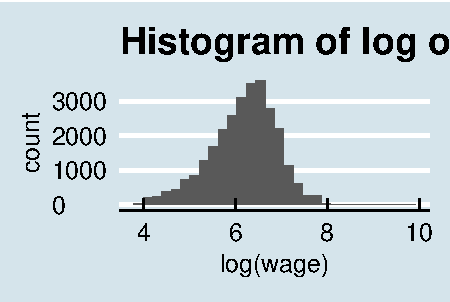
\includegraphics{Shortcourse_files/figure-latex/unnamed-chunk-7-1.pdf}

As we can see, the distribution of wages is quite skewed, and so we
might need to choose a distribution capable of generating highly skewed
outcomes. Another approach is to transform the data. In this case,
because all wages are positive, we could take their natural log. The
distribution of log wages appears to be far more normal than the initial
distribution, and it possible that the non-normality is explainable
using demographic characteristics.

\begin{Shaded}
\begin{Highlighting}[]
\KeywordTok{ggplot}\NormalTok{(CPS1988, }\KeywordTok{aes}\NormalTok{(}\DataTypeTok{x =} \KeywordTok{log}\NormalTok{(wage))) +}
\StringTok{  }\KeywordTok{geom_histogram}\NormalTok{() +}\StringTok{ }
\StringTok{  }\NormalTok{ggthemes::}\KeywordTok{theme_economist}\NormalTok{(}\DataTypeTok{base_size =} \DecValTok{12}\NormalTok{) +}
\StringTok{  }\KeywordTok{ggtitle}\NormalTok{(}\StringTok{"Histogram of log of wages"}\NormalTok{)}
\end{Highlighting}
\end{Shaded}

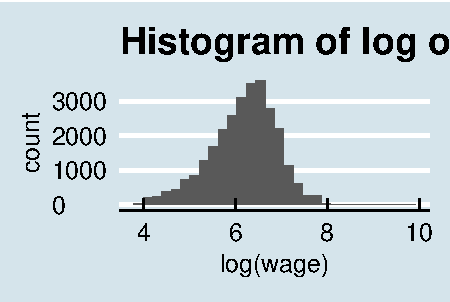
\includegraphics{Shortcourse_files/figure-latex/unnamed-chunk-8-1.pdf}

If we decide to choose a normal density as the data-generating process,
and assume that the conditional distribution of one person's wage does
not depend on the conditional distribution of another person's, we can
write it out like so:

\[
\log(\mbox{wage})_{i} \sim \mbox{Normal}(\mu_{i}, \sigma_{i})
\]

which says that a person \(i\)'s wage is distributed according to a
normal distribution with \emph{location} \(\mu_{i}\) and \emph{scale}
\(\sigma_{i}\). In the case of a normal density, the location is the
mean, and the scale is the standard deviation. We prefer to use
``location'' and ``scale'' rather than ``mean'' and ``standard
deviation'' because the terminology can carry across to other densities
whose location and scale parameters don't correspond to the mean or
standard deviation.

Let's be clear about what this means. This generative model says that
each individual's (log) wage is not completely determined---it involves
some amount of luck. So while on average it will be \(\mu_{i}\), luck
will result in differences from this average, and these differences have
a standard deviation of \(\sigma_{i}\).

Notice that both parameters \(\mu_{i}\) and \(\sigma_{i}\) vary across
each individual. One of the main challenges of building a good model is
to come up with functional forms for \(\mu_{i}\) and \(\sigma_{i}\),
taking into account the information available to us. For instance, the
(normal) linear regression model uses a (row) vector of individual
characteristics
\(X_{i} = (\mbox{education}_{i},\mbox{experience}_{i}, \dots)\), along
with a set of parameters that are common to all individuals (an
intercept \(\alpha\), coefficients \(\beta\) and a scale parameter
\(\sigma\)). The generative model is then:

\[
\log(\mbox{wage})_{i} \sim \mbox{Normal}(\alpha + X_{i}\beta, \sigma)
\] which is the same as saying:

\[
\log(\mbox{wage})_{i} = \alpha + X_{i}\beta + \epsilon_{i} \mbox{ with } \epsilon_{i} \sim \mbox{N}(0, \sigma)
\]

Note that we've made ``modeling assumptions''
\(\mu_{i} = \alpha + X_{i}\beta\) and \(\sigma_{i} = \sigma\). The
parameters of the generative model are both ``true'' and unknown. The
entire point is to peform inference in order to get probabilistic
estimates of the ``true'' parameters.

\subsubsection{Choosing the right generative
model}\label{choosing-the-right-generative-model}

Above, we picked out a normal density for log wages (which corresponds
to a lognormal density for wages) as a reasonable first step in modeling
our wage series. How did we get to this choice? The choice of
distribution to use should depend on the nature of your outcome
variables. Two good rules of thumb are:

\begin{enumerate}
\def\labelenumi{\arabic{enumi}.}
\tightlist
\item
  The chosen distribution should not give positive probability to
  impossible outcomes. For example, wages can't be negative, and so if
  we were to use a normal density (which gives positive probability to
  all outcomes) to model wages, we would be committing an error. If an
  outcome is outcome is binary or count data, the model should not give
  weight to non-integer outcomes. And so on.
\item
  The chosen distribution should give positive weight to plausible
  outcomes.
\end{enumerate}

\subsubsection{Choosing priors}\label{choosing-priors}

To complete our probability model, we need to specify priors for the
parameters \(\beta\) and \(\sigma\). Again, these priors should place
positive probabilistic weight over values of the parameters that we
consider possible, and zero weight on impossible values (like a negative
scale \(\sigma\)). In this case, it is common to assume normal priors
for regression coefficients and half-Cauchy or half-Student-t priors on
scales.

A great discussion of choosing priors is available
\href{github.com/stan-dev/wiki}{here}.

\subsubsection{Thinking ahead: are our data endogenous? Instrumental
variables}\label{thinking-ahead-are-our-data-endogenous-instrumental-variables}

As you will see in the generative model above, \(\epsilon\) are as
though they've been drawn from a (normal) random number generator, and
have no systematic relationship to the variables in X. Now what is the
economic meaning of \(\epsilon\)? The way I prefer to think about it is
as a catch-all containing the unobserved information that is relevant to
the outcome.

We need to think ahead: is there unobserved information that will be
systematically correlated with \(X\)? Can we tell a story that there are
things that cause both some change in one of our \(X\) variables and
also our observed wages? If such information exists, then at the model
estimation stage we will have an unobserved confounder problem, and we
need to consider it in our probability model. A common way of achiving
this is to use instrumental variables.

An instrumental variable is one that introduces plausible exogenous
variation into our endogenous regressor. For example, if we have years
of education on the right hand side, we might be concerned that the same
sorts of unobserved factors---family and peer pressure, IQ etc.---that
lead to high levels of education might also lead to high wages (even in
absense of high levels of education). In this case we would want to
``instrument'' education, ideally with an experimental treatment that
randomly assigned some people to higher rates of education and others to
less. In reality, such an experiment might not be possible to run, but
we might find ``natural experiments'' that result in the same variation.
The most famous case of such an instrument is the Vietnam war draft
(Angrist and Kreuger, 1992).

There are a few ways of incorporating instrumental variables. The first
is so-called ``two stage least squares'' in which we first regress the
endogenous regressor on the exogenous regressors (\(X_{edu,i}\)) plus an
instrument or instruments \(Z_{i}\). In the second stage we replace the
actual values of education with the fitted values from the first stage.

Stage one:

\[
\mbox{education}_{i} \sim \mbox{Normal}(\alpha_{s1} + X_{-edu,i}\gamma + Z_{i}\delta, \sigma_{s1})
\] Stage two:

\[
\log(wage_{i})  \sim \mbox{Normal}(\alpha_{s2} + X_{-edu,i}\beta + (\alpha_{s1} + X_{-edu,i}\gamma + Z_{i}\delta)\tau, \sigma_{s2})
\] (In the second stage, we only estimate \(\alpha_{s2}, \beta, \tau\)
and \(\sigma_{s2}\); the other parameters' values are from the first
stage).

If we treat the uncertainty of the first model approproately in the
second (as is automatic in Bayes), then two stage least squares yields
an consistent estimate of the treatment effect \(\tau\) (that is, as the
number of observations grows, we get less bias). But it may be
inefficient in the case when the residuals of the data generating
processes in stage one and stage two are correlated.

The second method of implementing instrumental variables is as a
simultaneous equations model. Under this framework, the generative model
is

\[
(\log(wage_{i}), \mbox{edu}_{i})' \sim \mbox{Multi normal}\left((\mu_{1,i}, \mu_{2, i})', \Sigma\right)
\] where

\[
\mu_{1,i} = \alpha_{s2} + X_{-edu,i}\beta + (\alpha_{s1} + X_{-edu,i}\gamma + Z_{i}\delta)\tau
\] and \[
\mu_{2,i} = \alpha_{s1} + X_{-edu,i}\gamma + Z_{i}\delta
\] You will see: this is the same as the two stage least squares model
above, exept we have allowed the errors to be correlated across
equations (this information is in the covariance matrix \(\Sigma\)).
Nobody really understands raw numbers from Covariance matrices, so we
typically decompose covariance into the more interpretable\\
scale vector \(\sigma\) and correlation matrix \(\Omega\) such that
\(\Sigma = \mbox{diag}(\sigma)\Omega \mbox{diag}(\sigma)\). This
decomposition also allows us to use more interpretable priors.

We now have two possible models. What we'll do below is simulate data
from the second model with known parmaters. Then we'll code up both
models and estimate each, allowing us to perform model comparison.

\subsection{Step 2: Simulating the model with known
parameters}\label{step-2-simulating-the-model-with-known-parameters}

We have now specified two probability models. What we will do next is
simulate some data from the second (more complex model), and then check
to see if we can recover the (known) model parameters by estimating both
the correctly specified and incorrectly specified models above.
Simulating and recovering known parameters is an important checking
procedure in model building; it often helps catch errors in the model
and clarifies the model in the mind of the modeler.

Now that we have written out the data generating model, let's generate
some known parameters and covariates and simulate the model. First:
generate some values for the data and paramaters.

\begin{Shaded}
\begin{Highlighting}[]
\CommentTok{# Generate a matrix of random numbers, and values for beta, nu and sigma}

\KeywordTok{set.seed}\NormalTok{(}\DecValTok{48}\NormalTok{) }\CommentTok{# Set the random number generator seed so that we get the same parameters}
\NormalTok{N <-}\StringTok{ }\DecValTok{500} \CommentTok{# Number of observations}
\NormalTok{P <-}\StringTok{ }\DecValTok{5} \CommentTok{# Number of covariates}
\NormalTok{X <-}\StringTok{ }\KeywordTok{matrix}\NormalTok{(}\KeywordTok{rnorm}\NormalTok{(N*P), N, P) }\CommentTok{# generate an N*P covariate matrix of random data}
\NormalTok{Z <-}\StringTok{ }\KeywordTok{rnorm}\NormalTok{(N) }\CommentTok{# an instrument}

\CommentTok{# The parameters governing the residuals}
\NormalTok{sigma <-}\StringTok{ }\KeywordTok{c}\NormalTok{(}\DecValTok{1}\NormalTok{, }\DecValTok{2}\NormalTok{)}
\NormalTok{Omega <-}\StringTok{ }\KeywordTok{matrix}\NormalTok{(}\KeywordTok{c}\NormalTok{(}\DecValTok{1}\NormalTok{, .}\DecValTok{5}\NormalTok{, .}\DecValTok{5}\NormalTok{, }\DecValTok{1}\NormalTok{), }\DecValTok{2}\NormalTok{, }\DecValTok{2}\NormalTok{)}

\CommentTok{# Generate some residuals}
\NormalTok{resid <-}\StringTok{ }\NormalTok{MASS::}\KeywordTok{mvrnorm}\NormalTok{(N, }\DataTypeTok{mu =} \KeywordTok{c}\NormalTok{(}\DecValTok{0}\NormalTok{, }\DecValTok{0}\NormalTok{), }\DataTypeTok{Sigma =} \KeywordTok{diag}\NormalTok{(sigma)%*%}\StringTok{ }\NormalTok{Omega %*%}\StringTok{ }\KeywordTok{diag}\NormalTok{(sigma))}

\CommentTok{# Now the parameters of our model}
\NormalTok{beta <-}\StringTok{ }\KeywordTok{rnorm}\NormalTok{(P)}
\NormalTok{tau <-}\StringTok{ }\DecValTok{1} \CommentTok{# This is the treatment effect we're looking to recover}
\NormalTok{alpha_1 <-}\StringTok{ }\KeywordTok{rnorm}\NormalTok{(}\DecValTok{1}\NormalTok{)}
\NormalTok{alpha_2 <-}\StringTok{ }\KeywordTok{rnorm}\NormalTok{(}\DecValTok{1}\NormalTok{)}
\NormalTok{gamma <-}\StringTok{ }\KeywordTok{rnorm}\NormalTok{(P)}
\NormalTok{delta <-}\StringTok{ }\KeywordTok{rnorm}\NormalTok{(}\DecValTok{1}\NormalTok{)}

\NormalTok{mu_2 <-}\StringTok{ }\NormalTok{alpha_1 +}\StringTok{ }\NormalTok{X%*%gamma +}\StringTok{ }\NormalTok{Z*delta}
\NormalTok{mu_1 <-}\StringTok{ }\NormalTok{alpha_2 +}\StringTok{ }\NormalTok{X%*%beta +}\StringTok{ }\NormalTok{mu_2*tau}

\NormalTok{Y <-}\StringTok{ }\KeywordTok{as.numeric}\NormalTok{(mu_1 +}\StringTok{ }\NormalTok{resid[,}\DecValTok{1}\NormalTok{])}
\NormalTok{endog_regressor <-}\StringTok{ }\KeywordTok{as.numeric}\NormalTok{(mu_2 +}\StringTok{ }\NormalTok{resid[,}\DecValTok{2}\NormalTok{])}

\CommentTok{# And let's check we can't recapture with simple OLS: }

\KeywordTok{lm}\NormalTok{(Y ~}\StringTok{ }\NormalTok{. +}\StringTok{ }\NormalTok{endog_regressor, }\DataTypeTok{data =} \KeywordTok{as.data.frame}\NormalTok{(X))}
\end{Highlighting}
\end{Shaded}

\subsection{Writing out the Stan model to recover known
parameters}\label{writing-out-the-stan-model-to-recover-known-parameters}

A Stan model is comprised of code blocks. Each block is a place for a
certain task. The bold blocks below must be present in all Stan programs
(even if they contain no arguments):

\begin{enumerate}
\def\labelenumi{\arabic{enumi}.}
\tightlist
\item
  \texttt{functions}, where we define functions to be used in the blocks
  below. This is where we will write out a random number generator that
  gives us draws from our assumed model.
\item
  \texttt{data}, declares the data to be used for the model
\item
  \texttt{transformed\ data}, makes transformations of the data passed
  in above
\item
  \texttt{parameters}, defines the unknowns to be estimated, including
  any restrictions on their values. 
\item
  \texttt{transformed\ parameters}, often it is preferable to work with
  transformations of the parameters and data declared above; in this
  case we define them here.
\item
  \texttt{model}, where the full probability model is defined.
\item
  \texttt{generated\ quantities}, generates a range of outputs from the
  model (posterior predictions, forecasts, values of loss functions,
  etc.).
\end{enumerate}

\begin{Shaded}
\begin{Highlighting}[]
\CommentTok{# In R:}
\CommentTok{# Load necessary libraries and set up multi-core processing for Stan}
\KeywordTok{options}\NormalTok{(}\DataTypeTok{warn=}\NormalTok{-}\DecValTok{1}\NormalTok{, }\DataTypeTok{message =}\NormalTok{-}\DecValTok{1}\NormalTok{)}
\KeywordTok{library}\NormalTok{(dplyr); }\KeywordTok{library}\NormalTok{(ggplot2); }\KeywordTok{library}\NormalTok{(rstan); }\KeywordTok{library}\NormalTok{(reshape2)}
\KeywordTok{options}\NormalTok{(}\DataTypeTok{mc.cores =} \NormalTok{parallel::}\KeywordTok{detectCores}\NormalTok{())}
\end{Highlighting}
\end{Shaded}

Now we have \(y\) and \(X\), and we want to estimate \(\beta\),
\(\sigma\) and, depending on the model, \(\nu\). We have two candidate
probability models that we want to estimate and check which one is a
more plausible model of the data. To do this, we need to specify both
models in Stan and then estimate them.

Let's jump straight in and define the incorrectly specified model. It is
incorrect in that we haven't properly accounted for the mutual
information in first and second stage regressions.

\begin{verbatim}
// saved as models/independent_iv.stan
// saved as models/independent_iv.stan
data {
  int N; // number of observations
  int P; // number of covariates
  matrix[N, P] X; //covariate matrix
  vector[N] Y; //outcome vector
  vector[N] endog_regressor; // the endogenous regressor
  vector[N] Z; // the instrument (which we'll assume is a vector)
}
parameters {
  vector[P] beta; // the regression coefficients
  vector[P] gamma;
  real tau;
  real delta;
  real alpha_1;
  real alpha_2;
  vector<lower = 0>[2] sigma; // the residual standard deviation
  corr_matrix[2] Omega;
}
transformed parameters {
  matrix[N, 2] mu;
  
  for(i in 1:N) {
    mu[i,2] = alpha_1 + X[i]*gamma + Z[i]*delta;
    mu[i,1] = alpha_2 + X[i]*beta + mu[i,2]*tau;
  }
}
model {
  // Define the priors
  beta ~ normal(0, 1); 
  gamma ~ normal(0, 1);
  tau ~ normal(0, 1);
  sigma ~ cauchy(0, 1);
  delta ~ normal(0, 1);
  alpha_1 ~ normal(0, 1);
  alpha_2 ~ normal(0, 2);
  Omega ~ lkj_corr(5);
  
  // The likelihood
  for(i in 1:N) {
    Y[i]~ normal(mu[i], sigma[1]);
    endog_regressor[i]~ normal(mu[2], sigma[2]);
  }

  
}
generated quantities {
  // For model comparison, we'll want to keep the likelihood
  // contribution of each point

  vector[N] log_lik;
  for(i in 1:N) {
    log_lik[i] = normal_lpdf(Y[i] | alpha_1  + X[i,] * beta + endog_regressor[i]*tau, sigma[1]);
  }
}
\end{verbatim}

Now we define the correctly specified model. It is the same as above,
but with a couple of changes:

\begin{verbatim}
// saved as models/joint_iv.stan
// saved as models/joint_iv.stan
data {
  int N; // number of observations
  int P; // number of covariates
  matrix[N, P] X; //covariate matrix
  vector[N] Y; //outcome vector
  vector[N] endog_regressor; // the endogenous regressor
  vector[N] Z; // the instrument (which we'll assume is a vector)
}
parameters {
  vector[P] beta; // the regression coefficients
  vector[P] gamma;
  real tau;
  real delta;
  real alpha_1;
  real alpha_2;
  vector<lower = 0>[2] sigma; // the residual standard deviation
  corr_matrix[2] Omega;
}
transformed parameters {
  matrix[N, 2] mu;
  
  for(i in 1:N) {
    mu[i,2] = alpha_1 + X[i]*gamma + Z[i]*delta;
    mu[i,1] = alpha_2 + X[i]*beta + mu[i,2]*tau;
  }
}
model {
  // Define the priors
  beta ~ normal(0, 1); 
  gamma ~ normal(0, 1);
  tau ~ normal(0, 1);
  sigma ~ cauchy(0, 1);
  delta ~ normal(0, 1);
  alpha_1 ~ normal(0, 1);
  alpha_2 ~ normal(0, 2);
  Omega ~ lkj_corr(5);
  
  // The likelihood
  {
    matrix[N, 2] Y2;
    Y2 = append_col(Y, endog_regressor);
    for(i in 1:N) {
      Y2[i]~ multi_normal(mu[i], diag_matrix(sigma)*Omega*diag_matrix(sigma));
    }
  }
  
}
generated quantities {
  // For model comparison, we'll want to keep the likelihood
  // contribution of each point

  vector[N] log_lik;
  for(i in 1:N) {
    log_lik[i] = normal_lpdf(Y[i] | alpha_1  + X[i,] * beta + endog_regressor[i]*tau, sigma[1]);
  }
}
\end{verbatim}

Now that we have specified two models, let's estimate them with the
\(y\) and \(X\) we generated above.

\begin{Shaded}
\begin{Highlighting}[]
\CommentTok{# In R}

\NormalTok{compiled_model <-}\StringTok{ }\KeywordTok{stan_model}\NormalTok{(}\StringTok{""}\NormalTok{)}

\NormalTok{incorrect_fit <-}\StringTok{ }\KeywordTok{stan}\NormalTok{(}\DataTypeTok{file =} \StringTok{"models/independent_iv.stan"}\NormalTok{,}
                      \DataTypeTok{data =} \KeywordTok{list}\NormalTok{(}\DataTypeTok{Y =} \NormalTok{Y,}
                                  \DataTypeTok{X =} \NormalTok{X,}
                                  \DataTypeTok{endog_regressor =} \NormalTok{endog_regressor,}
                                  \DataTypeTok{P =} \NormalTok{P, }
                                  \DataTypeTok{N =} \NormalTok{N,}
                                  \DataTypeTok{Z =} \NormalTok{Z), }
                      \DataTypeTok{iter =} \DecValTok{600}\NormalTok{)}

\NormalTok{correct_fit <-}\StringTok{ }\KeywordTok{stan}\NormalTok{(}\DataTypeTok{model_code =} \StringTok{"models/joint_iv.stan"}\NormalTok{,}
                    \DataTypeTok{data =} \KeywordTok{list}\NormalTok{(}\DataTypeTok{Y =} \NormalTok{Y,}
                                \DataTypeTok{X =} \NormalTok{X,}
                                \DataTypeTok{endog_regressor =} \NormalTok{endog_regressor,}
                                \DataTypeTok{P =} \NormalTok{P, }
                                \DataTypeTok{N =} \NormalTok{N,}
                                \DataTypeTok{Z =} \NormalTok{Z),}
                    \DataTypeTok{iter =} \DecValTok{600}\NormalTok{)}
\end{Highlighting}
\end{Shaded}

We have now fit our two competing models to the data. What has been
estimated?

\subsubsection{What do these fitted objects
contain?}\label{what-do-these-fitted-objects-contain}

If you are accustomed to estimating models using ordinary least squares
(OLS), maximum likelihood estimates (MLE), or the general method of
moments (GMM), then you may expect point estimates for parameters:
regression tables contain an estimate of the parameter along with some
standard errors. Full Bayesian inference involves averaging over the
uncertainty in parameter estimates, that is, the posterior distribution.
For a point estimate, Bayesians typically use the mean of the posterior
distribution, because it minimizes expected square error in the
estimate; the posterior median minimizes expected absolute error.

For all but a few models, posterior distributions cannot be expressed
analytically. Instead, numerical techniques involving simulation going
under the general heading of Monte Carlo methods, are used to estimate
quantities of interest by taking draws from the distribution in
question.

Monte Carlo estimation is quite simple. Let's say a parameter \(\theta\)
is distributed according to some distribution \(\mbox{Foo}(\theta)\) for
which we have no analytical formula, but from which we can simulate
random draws. We want to draw statistical inferences using this
distribution; we want its mean (expected value), standard deviation,
median and other quantiles for posterior intervals, etc. The Monte Carlo
method allows us to make these inferences by simply generating many (not
necessarily independent) draws from the distribution and then
calculating the statistic of interest from those draws. Because these
draws are from the distribution of interest, they will tend to come from
the higher probability regions of the distribution. For example, if 50\%
of the posterior probability mass is near the posterior mode, then 50\%
of the simulated draws (give or take sampling error) should be near the
posterior mode.

For example, suppose we want to estimate the expectation of
\(\mbox{Foo}(\theta)\), or in other words, the mean of a variable
\(\theta\) with distribution \(\mbox{Foo}(\theta)\). If we take \(M\)
random draws from \(\mbox{Foo}\), \[
\theta^{(1)}, \ldots, \theta^{(M)} \sim \mbox{Foo}(),
\] then we can estimate the expected value of \(\theta\) (i.e., its
posterior mean) as \[
\mathbb{E}[\theta]
\approx
\frac{1}{M} \sum_{m=1}^{M} \theta^{(m)}.
\]

If the draws \(\theta^{(m)}\) are independent, the result is a sequence
of independent and identically distributed (i.i.d.) draws. The mean of a
sequence of i.i.d. draws is governed by the central limit theorem, where
the standard error on the estimates is given by the standard deviation
divided by the square root of the number of draws. Thus standard error
decreases as \(\mathcal{O}(\frac{1}{\sqrt{M}})\) in the number of
independent draws \(M\).

What makes Bayesian inference not only possible, but practical, is that
almost all of the Bayesian inference for event probabilities,
predictions, and parameter estimates can be expressed as expectations
and carried out using Monte Carlo methods.

There is one hitch, though. For almost any practically useful model, not
only will we not be able to get an analytical formula for the posterior,
we will not be able to take independent draws. Fortunately, all is not
lost, as we will be able to take identically distributed draws using a
technique known as Markov chain Monte Carlo (MCMC). With MCMC, the draws
from a Markov chain in which each draw \(\theta^{(m+1)}\) depends (only)
on the previous draw \(\theta^{(m)}\). Such draws are governed by the
MCMC central limit theorem, wherein a quantity known as the effective
sample size plays the role of the effective sample size in pure Monte
Carlo estimation. The effective sample size is determined by how
autocorrelated the draws are; if each draw is highly correlated with
previous draws, then more draws are required to achieve the same
effective sample size.

Stan is able to calculate the effective sample size for its MCMC methods
and use that to estimate standard errors for all of its predictive
quantities, such as parameter and event probability estimates.

A fitted Stan object contains a sequence of \(M\) draws, where each draw
contains a value for every parameter (and generated quantity) in the
model. If the computation has converged, as measured by built-in
convergence diagnostics, the draws are from the posterior distribution
of our parameters conditioned on the observed data. These are draws from
the joint posterior distribution; correlation between parameters is
likely to be present in the joint posterior even if it was not present
in the priors.

In the generated quantities block of the two models above, we declare
variables for two additional quantities of interest.

\begin{itemize}
\item
  The first, \texttt{log\_lik}, is the log-likelihood, which we use for
  model comparison. We obtain this value for each parameter draw, for
  each value of \(y_{i}\). Thus if you have \(N\) observations and
  \texttt{iter} parameter draws, this will contain \(N\times\)
  \texttt{iter} log-likelihood values (which may produce a lot of output
  for large data sets).
\item
  The second, \texttt{y\_sim}, is a \emph{posterior predictive
  quantity}, in this case a replicated data set consisting of a sequence
  of fresh outcomes generated randomly from the parameters. Rather than
  each observation having a ``predicted value'', it has a predictive
  distribution that takes into account both the regression residual and
  uncertainty in the parameter estimates.
\end{itemize}

\subsection{Model inspection}\label{model-inspection}

To address questions 1 and 2 above, we need to examine the parameter
draws from the model to check for a few common problems:

\begin{itemize}
\tightlist
\item
  \textbf{Lack of mixing}. A poorly ``mixing'' Markov chain is one that
  moves very slowly between regions of the parameter space or barely
  moves at all. This can happen if the distribution of proposals is much
  narrower than the target (posterior) distribution or if it is much
  wider than the target distribution. In the former case most proposals
  will be accepted but the Markov chain will not explore the full
  parameter space whereas in the latter case most proposals will be
  rejected and the chain will stall. By running several Markov chains
  from different starting values we can see if each chain mixes well and
  if the chains are converging on a common distribution. If the chains
  don't mix well then it's unlikely we're sampling from a well specified
  posterior. The most common reason for this error is a poorly specified
  model.
\item
  \textbf{Stationarity}. Markov chains should be covariance stationary,
  which means that the mean and variance of the chain should not depend
  on when you draw the observations. Non-stationarity is normally the
  consequence of a poorly specified model or an insufficient number of
  iterations.
\item
  \textbf{Autocorrelation}. Especially in poorly specified or weakly
  identified models, a given draw of parameters can be highly dependent
  on the previous draw of the parameters. One consequence of
  autocorrelation is that the posterior draws will contain less
  information than the number of draws suggests. That is, the effective
  posterior sample size will be much less than the actual posterior
  sample size. For example, 2000 draws with high autocorrelation will be
  less informative than 2000 independent draws. Assuming the model is
  specified correctly, then \emph{thinning} (keeping only every k-th
  draw) is one common approach to dealing with highly autocorrelated
  draws. However, while thinning can reduce the autocorrelation in the
  draws that are retained it still sacrifices information. If possible,
  \href{http://mc-stan.org/documentation/}{reparameterising the model}
  is a better approach to this problem. (See section 21 of the manual,
  on Optimizing Stan code).
\item
  \textbf{Divergent transitions}. In models with very curved or
  irregular posterior densities, we often get ``divergent transitions''.
  This typically indicates that the sampler was unable to explore
  certain regions of the distribution and a respecification or changes
  to the sampling routine may be required. The easiest way of addressing
  this issue is to use \texttt{control\ =\ list(adapt\_delta\ =\ 0.99)}
  or some other number close to 1. This will lead to smaller step sizes
  and therefore more steps will be required to explore the posterior.
  Sampling will be slower but the algorithm will often be better able to
  explore these problematic regions, reducing the number of divergent
  transitions.
\end{itemize}

All of these potential problems can be checked using the ShinyStan
graphical interface, which is available in the \texttt{shinystan}
\texttt{R} package. You can install it with
\texttt{install.packages("shinystan")}, and run it with
\texttt{launch\_shinystan(correct\_fit)}. It will bring up an
interactive session in your web browser within which you can explore the
estimated parameters, examine the individual Markov chains, and check
various diagnostics. More information on ShinyStan is available
\href{http://mc-stan.org/interfaces/shinystan}{here}. We will confront
most of these issues and show how to resolve them in later chapters when
we work with real examples. For now just keep in mind that MCMC samples
always need to be checked before they are used for making inferences.

\subsection{Model comparison}\label{model-comparison}

Let's start by looking at the model outputs. The draws from each
parameter can be neatly summarized with \texttt{print}:

\begin{Shaded}
\begin{Highlighting}[]
\CommentTok{# In R:}

\KeywordTok{print}\NormalTok{(incorrect_fit, }\DataTypeTok{pars =} \KeywordTok{c}\NormalTok{(}\StringTok{"beta"}\NormalTok{, }\StringTok{"tau"}\NormalTok{, }\StringTok{"sigma"}\NormalTok{))}
\CommentTok{# specify parameters to save; else we'd get `log_lik` and `y_sim`}

\CommentTok{# Some things to note:}

\CommentTok{# - mean is the mean of the draws for each observation}
\CommentTok{# - se_mean is the Monte Carlo error}
\CommentTok{#   (standard error of the Monte Carlo estimate from the true mean)}
\CommentTok{# - sd is the standard deviation of the parameter's draws}
\CommentTok{# - the quantiles are self-explanatory}
\CommentTok{# - n_eff is the effective number of independent draws.}
\CommentTok{#   If there is serial correlation between sequential draws,}
\CommentTok{#   the draws cannot be considered independent.}
\CommentTok{#   In Stan, high serial correlation is typically a problem in}
\CommentTok{#   poorly specified models}
\CommentTok{# - Rhat: this is the Gelman Rubin convergence diagnostic.}
\CommentTok{#   Values close to 1 indicate that the multiple chains}
\CommentTok{#   that you estimated have converged to the same}
\CommentTok{#   distribution and are "mixing" well.}
\end{Highlighting}
\end{Shaded}

\begin{Shaded}
\begin{Highlighting}[]
\CommentTok{# In R}

\KeywordTok{print}\NormalTok{(correct_fit, }\DataTypeTok{pars =} \KeywordTok{c}\NormalTok{(}\StringTok{"beta"}\NormalTok{, }\StringTok{"sigma"}\NormalTok{, }\StringTok{"nu"}\NormalTok{))}
\end{Highlighting}
\end{Shaded}

At the moment, it seems as though both our models have done about as
good a job at estimating the regression coefficients \(\beta\) as one
another. But the incorrectly specified model severely overestimates
\(\sigma\). This makes sense--a Student-t distribution with \(\nu=5\)
will have fat tails, and so a normal distribution will try to replicate
the extreme values by having a large variance.

How else might we compare the two models?

One approach is to use the \texttt{loo} package to compare the models on
their estimated out-of-sample predictive performance. The idea of this
package is to approximate each model's leave-one-out (LOO)
cross-validation error, allowing model comparison by the LOO Information
Criterion (LOOIC). LOOIC has the same purpose as the Akaike Information
Criterion (AIC), which is to estimate the expected log predictive
density (ELPD) for a new dataset. However, AIC ignores prior
distributions and makes the assumption that the posterior is a
multivariate normal distribution. The approach taken by the \texttt{loo}
package does not make this distributional assumption and also integrates
over (averages over) the uncertainty in the parameters.

The Bayesian LOO estimate is
\(\sum_{n = 1}^{N}\log p(y_{n} \, | \, y_{1}, ..., y_{n-1}, y_{n+1}, ..., y_{N})\),
which requires fitting the model \(N\) times, each time leaving out one
of the \(N\) data points. For large datasets or complex models the
computational cost is usually prohibitive. The \texttt{loo} package does
an approximation that avoids re-estimating the model and requires only
the log-likelihood evaluated at the posterior draws of the parameters.
The approximation will be good so long as the posterior distribution is
not very sensitive to leaving out any single observation.

A big upside of this approach is that it enables us to generate
probabilistic estimates of the degree to which each model is most likely
to produce the best out-of-sample predictions.

We use \texttt{loo} like so:

\begin{Shaded}
\begin{Highlighting}[]
\CommentTok{# in R}
\CommentTok{# }
\CommentTok{# library(loo) # Load the library}
\CommentTok{# }
\CommentTok{# # Extract the log likelihoods of both models.}
\CommentTok{# # Note that we need to declare log_lik in the generated quantities block}
\NormalTok{llik_incorrect <-}\StringTok{ }\KeywordTok{extract_log_lik}\NormalTok{(incorrect_fit, }\DataTypeTok{parameter_name =} \StringTok{"log_lik"}\NormalTok{)}
\NormalTok{llik_correct <-}\StringTok{ }\KeywordTok{extract_log_lik}\NormalTok{(correct_fit, }\DataTypeTok{parameter_name =} \StringTok{"log_lik"}\NormalTok{)}
\CommentTok{# }
\CommentTok{# # Estimate the leave-one-out cross validation error}
\NormalTok{loo_incorrect <-}\StringTok{ }\KeywordTok{loo}\NormalTok{(llik_incorrect)}
\NormalTok{loo_correct <-}\StringTok{ }\KeywordTok{loo}\NormalTok{(llik_correct)}
\end{Highlighting}
\end{Shaded}

\begin{Shaded}
\begin{Highlighting}[]
\CommentTok{# # Print the LOO statistics}
\KeywordTok{print}\NormalTok{(}\StringTok{"Incorrect model"}\NormalTok{)}
\KeywordTok{print}\NormalTok{(loo_incorrect)}
\end{Highlighting}
\end{Shaded}

\begin{Shaded}
\begin{Highlighting}[]
\KeywordTok{print}\NormalTok{(}\StringTok{"Correct model"}\NormalTok{)}
\KeywordTok{print}\NormalTok{(loo_correct)}
\end{Highlighting}
\end{Shaded}

The quantity \texttt{elpd\_loo} is the expected log pointwise predictive
density (ELPD). The log pointwise predictive density is easiest to
understand in terms of its computation. For each data point we compute
the log of its average likelihood, where the average is computed over
the posterior draws. Then we take the sum over all of the data points.
We can multiply \texttt{elpd\_loo} by \(-2\) to calculate the
\texttt{looic}, which you can think of like AIC or BIC, but coming from
our Bayesian framework. The \(-2\) is not important; it simply converts
the value to the so-called deviance scale. The value of \texttt{p\_loo}
is the estimated effective number of parameters, which is a measure of
model complexity. The effective number of parameters can be
substantially less than the actual number of parameters when there is
strong dependence between parameters (e.g.~in many hierarchical models)
or when parameters are given informative prior distributions. For
further details on these quantities, please consult
\href{http://arxiv.org/abs/1507.04544}{this paper}.

\begin{Shaded}
\begin{Highlighting}[]
\CommentTok{# Print the comparison between the two models}
\KeywordTok{print}\NormalTok{(}\KeywordTok{compare}\NormalTok{(loo_incorrect, loo_correct), }\DataTypeTok{digits =} \DecValTok{2}\NormalTok{)}
\end{Highlighting}
\end{Shaded}

When using the \texttt{compare} function to compare two models the
\texttt{elpd\_diff} gives us the difference in the ELPD estimates for
the models. A positive \texttt{elpd\_diff} indicates that the second
model is estimated to have better out-of-sample predictive accuracy than
the first, which is precisely what we expect in this case. When
comparing more than two models the \texttt{compare} function will order
the models by their ELPD estimates.

\section{Tools of the trade: borrowing from software
engineering}\label{tools-of-the-trade-borrowing-from-software-engineering}

Building economic and statistical models increasingly requires
sophisticated computation. This has the potential to improve our
modeling, but carries with it risks; as the complexity of our models
grows, so too does the prospect of making potentially influential
mistakes. The well-known spreadsheet error in Rogoff and Reinhart's
(Cite) paper---a fairly simple error in very public paper---was
discovered. Who knows how many other errors exist in more complex, less
scruitinized work?

Given the ease of making errors that substantively affect our models'
outputs, it makes sense to adopt a workflow that minimizes the risk of
such error happening. The set of tools discussed in this section, all
borrowed from software engineering, are designed for this purpose. We
suggest incorporating the following into your workflow:

\begin{itemize}
\tightlist
\item
  Document your code formally. At the very least, this will involve
  commenting your code to the extend where a colleague could read it and
  not have too many questions. Ideally it will include formal
  documentation of every function that you write.
\item
  When you write functions, obey what we might call ``Tinbergen's rule
  of writing software'': \emph{one function, one objective}. Try not to
  write omnibus functions that conduct a large part of your analysis.
  Writing small, modular functions will allow you to use \textbf{unit
  testing}, a framework that lets you run a set of tests automatically,
  ensuring that changing one part of your code base does not break other
  parts.
\item
  Use Git to manage your workflow. Git is a very powerful tool that
  serves several purposes. It can help you back up your work, which is
  handy. It also allows you to view your codebase at periods when you
  \emph{committed} some code to the code base. It lets you experiment on
  \emph{branches}, without risking the main (``production'') code base.
  Finally helps you work in teams; formalizing a \textbf{code-review}
  procedure that should help catch errors.
\end{itemize}

\chapter{A more difficult model}\label{funtimeseries}

\section{This session}\label{this-session}

In this session, we'll cover two of the things that Stan lets you do
quite simply: implement state space models, and finite mixtures.

\subsection{Finite mixtures}\label{finite-mixtures}

In a post
\href{https://modernstatisticalworkflow.blogspot.com/2016/10/finite-mixture-models-in-stan.html}{here},
I describe a simple model in which each observation of our data could
have one of two densities. We estimated the parameters of both
densities, and the probability of the data coming from either. While
finite mixture models as in the last post are a useful learning aid, we
might want richer models for applied work. In particular, we might want
the probability of our data having each density to vary across
observations. This is the first of two posts dedicated to this topic. I
gave a
\href{https://dl.dropboxusercontent.com/u/63100926/become_a_bayesian_shareable.html}{talk}
covering some of this also (best viewed in Safari).

For sake of an example, consider this: the daily returns series of a
stock has two states. In the first, the stock is `priced to perfection',
and so the price is an I(1) random walk (daily returns are mean
stationary). In the second, there is momentum---here, daily returns have
AR(1) structure. Explicitly, for daily log returns \(r_{t}\):

State 1: \(r_{t} \sim \mbox{normal}(\alpha_{1}, \sigma_{1})\)

State 2:
\(r_{t} \sim \mbox{normal}(\alpha_{2} + \rho_{1} r_{t-1}, \sigma_{2})\)

When we observe a value of \(r_{t}\), we don't know for sure whether it
came from the first or second model--that is precisely what we want to
infer. For this, we need a model for the probability that an observation
came from each state \(s_{t}\in 1, 2\). One such model could be:

\[
\mbox{prob}(s_{t}=1 | \mathcal{I}_{t}) = \mbox{Logit}^{-1}(\mu_{t})
\]

with

\[
\mu_{t} \sim \mbox{normal}(\alpha_{3} + \rho_{2}\mu_{t-1} + f(\mathcal{I}_{t}), \sigma_{3})
\]

Here, \(f(\mathcal{I}_{t})\) is a function of the information available
at the beginning of day \(t\). If we had interesting information about
sentiment, or news etc., it could go in here. For simplicity, let's say
\(f(\mathcal{I}_{t}) = \beta r_{t-1}\).

Under this specification (and for a vector containing all parameters,
\(\theta\)), we can specify the likelihood contribution of an
observation. It is simply the weighted average of likelihoods under each
candidate data generating process, where the weights are the
probabilities that the data comes from each density.

\[
p(r_{t} | \theta) = \mbox{Logit}^{-1}(\mu_{t})\, \mbox{normal}(r_{t}|\, \alpha_{1}, \sigma_{1}) + (1-\mbox{Logit}^{-1}(\mu_{t}))\, \mbox{normal}(r_{t}|\, \alpha_{2} + \rho r_{t-1}, \sigma_{2})
\]

As discussed in the last post, we work in log likelihoods, not
likelihoods. This means we should use the \texttt{log\_sum\_exp()}
function in Stan. This means that we express the log likelihood
contribution of a single point as:

\begin{Shaded}
\begin{Highlighting}[]
\KeywordTok{log_sum_exp}\NormalTok{(}\KeywordTok{log}\NormalTok{(}\KeywordTok{inv_logit}\NormalTok{(mu[t])) +}\StringTok{ }\KeywordTok{normal_lpdf}\NormalTok{(r[t] |}\StringTok{ }\NormalTok{alpha[}\DecValTok{1}\NormalTok{], sigma[}\DecValTok{1}\NormalTok{]),}
            \KeywordTok{log}\NormalTok{((}\DecValTok{1} \NormalTok{-}\StringTok{ }\KeywordTok{inv_logit}\NormalTok{(mu[t]))) +}\StringTok{ }\KeywordTok{normal_lpdf}\NormalTok{(r[t] |}\StringTok{ }\NormalTok{alpha[}\DecValTok{2}\NormalTok{] +}\StringTok{ }\NormalTok{rho[}\DecValTok{1}\NormalTok{], sigma[}\DecValTok{2}\NormalTok{]))}
\end{Highlighting}
\end{Shaded}

Stan has recently added another function which performs the same
calculation, but makes writing it out a bit easier. For two log
densities \texttt{lp1}, \texttt{lp2} and a mixing probability
\texttt{theta}, we have

\begin{Shaded}
\begin{Highlighting}[]
\KeywordTok{log_mix}\NormalTok{(theta, lp1, lp2) =}\StringTok{ }\KeywordTok{log_sum_exp}\NormalTok{(}\KeywordTok{log}\NormalTok{(theta) +}\StringTok{ }\NormalTok{lp1,}
                                       \KeywordTok{log}\NormalTok{(}\DecValTok{1}\NormalTok{-theta) +}\StringTok{ }\NormalTok{lp2)}
\end{Highlighting}
\end{Shaded}

\subsection{Writing out the model}\label{writing-out-the-model}

The Stan code for the model is:

\begin{Shaded}
\begin{Highlighting}[]
\NormalTok{/}\ErrorTok{/}\StringTok{ }\NormalTok{saved as time_varying_finite_mixtures.stan}
\NormalTok{data \{}
  \NormalTok{int T;}
  \NormalTok{vector[T] r;}
\NormalTok{\}}
\NormalTok{parameters \{}
  \NormalTok{vector[T] mu;}
  \NormalTok{vector[}\DecValTok{2}\NormalTok{] rho;}
  \NormalTok{real beta;}
  \NormalTok{vector<lower =}\StringTok{ }\DecValTok{0}\NormalTok{>[}\DecValTok{3}\NormalTok{] sigma;}
  \NormalTok{vector[}\DecValTok{3}\NormalTok{] alpha; }
\NormalTok{\}}
\NormalTok{model \{}
  \NormalTok{/}\ErrorTok{/}\StringTok{ }\NormalTok{priors }
  \NormalTok{mu[}\DecValTok{1}\NormalTok{] ~}\StringTok{ }\KeywordTok{normal}\NormalTok{(}\DecValTok{0}\NormalTok{, .}\DecValTok{1}\NormalTok{);}
  \NormalTok{sigma ~}\StringTok{ }\KeywordTok{cauchy}\NormalTok{(}\DecValTok{0}\NormalTok{, }\FloatTok{0.5}\NormalTok{);}
  \NormalTok{rho ~}\StringTok{ }\KeywordTok{normal}\NormalTok{(}\DecValTok{1}\NormalTok{, .}\DecValTok{1}\NormalTok{);}
  \NormalTok{beta~}\StringTok{ }\KeywordTok{normal}\NormalTok{(.}\DecValTok{5}\NormalTok{, .}\DecValTok{25}\NormalTok{);}
  \NormalTok{alpha[}\DecValTok{1}\NormalTok{:}\DecValTok{2}\NormalTok{] ~}\StringTok{ }\KeywordTok{normal}\NormalTok{(}\DecValTok{0}\NormalTok{, }\FloatTok{0.1}\NormalTok{);}
  \NormalTok{alpha[}\DecValTok{3}\NormalTok{] ~}\StringTok{ }\KeywordTok{normal}\NormalTok{(}\DecValTok{0}\NormalTok{, }\DecValTok{1}\NormalTok{);}

  \NormalTok{/}\ErrorTok{/}\StringTok{ }\NormalTok{likelihood}
  \NormalTok{for(t in }\DecValTok{2}\NormalTok{:T) \{}
    \NormalTok{mu[t] ~}\StringTok{ }\KeywordTok{normal}\NormalTok{(alpha[}\DecValTok{3}\NormalTok{] +}\StringTok{ }\NormalTok{rho[}\DecValTok{1}\NormalTok{]*mu[t}\DecValTok{-1}\NormalTok{] +}\StringTok{ }\NormalTok{beta*}\StringTok{ }\NormalTok{r[t}\DecValTok{-1}\NormalTok{], sigma[}\DecValTok{3}\NormalTok{]);}

    \NormalTok{target +}\ErrorTok{=}\StringTok{ }\KeywordTok{log_mix}\NormalTok{(}\KeywordTok{inv_logit}\NormalTok{(mu[t]), }
                      \KeywordTok{normal_lpdf}\NormalTok{(r[t] |}\StringTok{ }\NormalTok{alpha[}\DecValTok{1}\NormalTok{], sigma[}\DecValTok{1}\NormalTok{]), }
                      \KeywordTok{normal_lpdf}\NormalTok{(r[t] |}\StringTok{ }\NormalTok{alpha[}\DecValTok{2}\NormalTok{] +}\StringTok{ }\NormalTok{rho[}\DecValTok{2}\NormalTok{] *}\StringTok{ }\NormalTok{r[t}\DecValTok{-1}\NormalTok{], sigma[}\DecValTok{2}\NormalTok{]));}
  \NormalTok{\}}
\NormalTok{\}}
\end{Highlighting}
\end{Shaded}

\subsection{\texorpdfstring{Recapturing `known
unknowns'}{Recapturing known unknowns}}\label{recapturing-known-unknowns}

As should be clear by now, I believe strongly that we should simulate
from the model and make sure that we can recapture ``known unknowns''
before taking the model to real data. Below we simulate some fake data.

\begin{Shaded}
\begin{Highlighting}[]
\CommentTok{# Set some fake parameters}
\NormalTok{alpha1 <-}\StringTok{ }\NormalTok{-}\FloatTok{0.01}
\NormalTok{alpha2 <-}\StringTok{ }\FloatTok{0.015}
\NormalTok{rho1 <-}\StringTok{ }\FloatTok{0.95}
\NormalTok{rho2 <-}\StringTok{ }\FloatTok{0.8}
\NormalTok{beta <-}\StringTok{ }\FloatTok{0.5}

\NormalTok{sigma1 <-}\StringTok{ }\FloatTok{0.05}
\NormalTok{sigma2 <-}\StringTok{ }\FloatTok{0.03}
\NormalTok{sigma3 <-}\StringTok{ }\FloatTok{0.3}
\NormalTok{T <-}\StringTok{ }\DecValTok{500}
\NormalTok{r <-}\StringTok{ }\KeywordTok{rep}\NormalTok{(}\OtherTok{NA}\NormalTok{, T)}
\NormalTok{r[}\DecValTok{1}\NormalTok{] <-}\StringTok{ }\DecValTok{0}

\NormalTok{mu <-}\StringTok{ }\KeywordTok{rep}\NormalTok{(}\OtherTok{NA}\NormalTok{, T)}
\NormalTok{z <-}\StringTok{ }\KeywordTok{rep}\NormalTok{(}\OtherTok{NA}\NormalTok{, T)}
\NormalTok{mu[}\DecValTok{1}\NormalTok{] <-}\StringTok{ }\DecValTok{0}
\NormalTok{z[}\DecValTok{1}\NormalTok{] <-}\StringTok{ }\DecValTok{1}


\CommentTok{# Simulate the data series}
\NormalTok{for(t in }\DecValTok{2}\NormalTok{:T) \{}
  \NormalTok{mu[t]  <-}\StringTok{ }\NormalTok{rho1 *}\StringTok{ }\NormalTok{mu[t}\DecValTok{-1}\NormalTok{] +}\StringTok{ }\NormalTok{beta*(r[t}\DecValTok{-1}\NormalTok{]) +}\StringTok{ }\KeywordTok{rnorm}\NormalTok{(}\DecValTok{1}\NormalTok{, }\DecValTok{0}\NormalTok{, sigma3)}
  \NormalTok{prob <-}\StringTok{ }\NormalTok{arm::}\KeywordTok{invlogit}\NormalTok{(mu[t])}
  \NormalTok{z[t] <-}\StringTok{ }\KeywordTok{sample}\NormalTok{(}\DecValTok{1}\NormalTok{:}\DecValTok{2}\NormalTok{, }\DecValTok{1}\NormalTok{, }\DataTypeTok{prob =} \KeywordTok{c}\NormalTok{(prob, }\DecValTok{1}\NormalTok{-prob))}
  
  \NormalTok{if(z[t]==}\DecValTok{1}\NormalTok{) \{}
    \CommentTok{# random walk state}
    \NormalTok{r[t] <-}\StringTok{ }\KeywordTok{rnorm}\NormalTok{(}\DecValTok{1}\NormalTok{, alpha1, sigma1)}
  \NormalTok{\} else \{}
    \CommentTok{# momentum state}
    \NormalTok{r[t] <-}\StringTok{ }\KeywordTok{rnorm}\NormalTok{(}\DecValTok{1}\NormalTok{, alpha2 +}\StringTok{ }\NormalTok{rho2*r[t}\DecValTok{-1}\NormalTok{], sigma2)}
  \NormalTok{\}}
\NormalTok{\}}
\end{Highlighting}
\end{Shaded}

You should plot your data before doing anything. Let's take a look.

\begin{Shaded}
\begin{Highlighting}[]
\CommentTok{# Plot the returns}
\KeywordTok{plot.ts}\NormalTok{(r)}
\CommentTok{# Plot the probability of the random walk state}
\KeywordTok{plot.ts}\NormalTok{(arm::}\KeywordTok{invlogit}\NormalTok{(mu))}
\end{Highlighting}
\end{Shaded}

Looks good! Now we compile and run the model.

\begin{Shaded}
\begin{Highlighting}[]
\NormalTok{compiled_model <-}\StringTok{ }\KeywordTok{stan_model}\NormalTok{(}\StringTok{"time_varying_finite_mixtures.stan"}\NormalTok{)}

\NormalTok{estimated_model <-}\StringTok{ }\KeywordTok{sampling}\NormalTok{(compiled_model, }\DataTypeTok{data =} \KeywordTok{list}\NormalTok{(}\DataTypeTok{r =} \NormalTok{r, }\DataTypeTok{T =} \NormalTok{T), }\DataTypeTok{cores =} \DecValTok{4}\NormalTok{, }\DataTypeTok{chains =} \DecValTok{4}\NormalTok{)}
\end{Highlighting}
\end{Shaded}

Now we inspect the parameter estimates, which should align with those in
our data generating process.

\begin{Shaded}
\begin{Highlighting}[]
\KeywordTok{print}\NormalTok{(estimated_model, }\DataTypeTok{pars =} \KeywordTok{c}\NormalTok{(}\StringTok{"alpha"}\NormalTok{, }\StringTok{"rho"}\NormalTok{, }\StringTok{"sigma"}\NormalTok{))}
\end{Highlighting}
\end{Shaded}

It seems that most of the parameters appear to have estimated quite
cleanly--most of the Rhats are fairly close, to 1, with the exception of
the standard deviation of the updates in the latent series (which will
be very weakly identified, given we don't observe \texttt{mu}). We would
fix this by adding better prior information to the model.

\subsection{Taking the model to real
data}\label{taking-the-model-to-real-data}

Now we know that our program can recapture a known model, we can take it
to some real data. In this case, we'll use the log differences in
sequential adjusted closing prices for Apple's common stock. With Apple
being such a large, well-researched (and highly liquid) stock, we should
expect that it spends almost all time in the random walk state. Let's
see what the data say!

\begin{Shaded}
\begin{Highlighting}[]
\CommentTok{# Now with real data! }
\NormalTok{aapl <-}\StringTok{ }\NormalTok{Quandl::}\KeywordTok{Quandl}\NormalTok{(}\StringTok{"YAHOO/AAPL"}\NormalTok{)}

\NormalTok{aapl <-}\StringTok{ }\NormalTok{aapl %>%}
\StringTok{  }\KeywordTok{mutate}\NormalTok{(}\DataTypeTok{Date =} \KeywordTok{as.Date}\NormalTok{(Date)) %>%}
\StringTok{  }\KeywordTok{arrange}\NormalTok{(Date) %>%}\StringTok{ }
\StringTok{  }\KeywordTok{mutate}\NormalTok{(}\DataTypeTok{l_ac =} \KeywordTok{log}\NormalTok{(}\StringTok{`}\DataTypeTok{Adjusted Close}\StringTok{`}\NormalTok{),}
         \DataTypeTok{dl_ac =} \KeywordTok{c}\NormalTok{(}\OtherTok{NA}\NormalTok{, }\KeywordTok{diff}\NormalTok{(l_ac))) %>%}\StringTok{ }
\StringTok{  }\KeywordTok{filter}\NormalTok{(Date >}\StringTok{ "2015-01-01"}\NormalTok{)}

\NormalTok{aapl_mod <-}\StringTok{ }\KeywordTok{sampling}\NormalTok{(compiled_model, }\DataTypeTok{data=} \KeywordTok{list}\NormalTok{(}\DataTypeTok{T =} \KeywordTok{nrow}\NormalTok{(aapl), }\DataTypeTok{r =} \NormalTok{aapl$dl_ac*}\DecValTok{100}\NormalTok{))}
\end{Highlighting}
\end{Shaded}

Now check that the model has fit properly

\begin{Shaded}
\begin{Highlighting}[]
\NormalTok{shinystan::}\KeywordTok{launch_shinystan}\NormalTok{(aapl_mod)}
\end{Highlighting}
\end{Shaded}

And finally plot the probability of being in each state.

\begin{Shaded}
\begin{Highlighting}[]
\NormalTok{plot1 <-}\StringTok{ }\NormalTok{aapl_mod %>%}\StringTok{ }
\StringTok{  }\KeywordTok{as.data.frame}\NormalTok{() %>%}\StringTok{ }
\StringTok{  }\KeywordTok{select}\NormalTok{(}\KeywordTok{contains}\NormalTok{(}\StringTok{"mu"}\NormalTok{)) %>%}
\StringTok{  }\KeywordTok{melt}\NormalTok{() %>%}\StringTok{ }
\StringTok{  }\KeywordTok{group_by}\NormalTok{(variable) %>%}\StringTok{ }
\StringTok{  }\KeywordTok{summarise}\NormalTok{(}\DataTypeTok{lower =} \KeywordTok{quantile}\NormalTok{(value, }\FloatTok{0.95}\NormalTok{), }
            \DataTypeTok{median =} \KeywordTok{median}\NormalTok{(value),}
            \DataTypeTok{upper =} \KeywordTok{quantile}\NormalTok{(value, }\FloatTok{0.05}\NormalTok{)) %>%}\StringTok{ }
\StringTok{  }\KeywordTok{mutate}\NormalTok{(}\DataTypeTok{date =} \NormalTok{aapl$Date,}
         \DataTypeTok{ac =} \NormalTok{aapl$l_ac) %>%}
\StringTok{  }\KeywordTok{ggplot}\NormalTok{(}\KeywordTok{aes}\NormalTok{(}\DataTypeTok{x =} \NormalTok{date)) +}\StringTok{ }
\StringTok{  }\KeywordTok{geom_ribbon}\NormalTok{(}\KeywordTok{aes}\NormalTok{(}\DataTypeTok{ymin =} \NormalTok{arm::}\KeywordTok{invlogit}\NormalTok{(lower), }\DataTypeTok{ymax =} \NormalTok{arm::}\KeywordTok{invlogit}\NormalTok{(upper)), }\DataTypeTok{fill=} \StringTok{"orange"}\NormalTok{, }\DataTypeTok{alpha =} \FloatTok{0.4}\NormalTok{) +}
\StringTok{  }\KeywordTok{geom_line}\NormalTok{(}\KeywordTok{aes}\NormalTok{(}\DataTypeTok{y =} \NormalTok{arm::}\KeywordTok{invlogit}\NormalTok{(median))) +}
\StringTok{  }\NormalTok{ggthemes::}\KeywordTok{theme_economist}\NormalTok{() +}
\StringTok{  }\KeywordTok{xlab}\NormalTok{(}\StringTok{"Date"}\NormalTok{) +}
\StringTok{  }\KeywordTok{ylab}\NormalTok{(}\StringTok{"Probability of random walk model"}\NormalTok{)}


\NormalTok{plot2 <-}\StringTok{ }\NormalTok{aapl_mod %>%}\StringTok{ }
\StringTok{  }\KeywordTok{as.data.frame}\NormalTok{() %>%}\StringTok{ }
\StringTok{  }\KeywordTok{select}\NormalTok{(}\KeywordTok{contains}\NormalTok{(}\StringTok{"mu"}\NormalTok{)) %>%}
\StringTok{  }\KeywordTok{melt}\NormalTok{() %>%}\StringTok{ }
\StringTok{  }\KeywordTok{group_by}\NormalTok{(variable) %>%}\StringTok{ }
\StringTok{  }\KeywordTok{summarise}\NormalTok{(}\DataTypeTok{lower =} \KeywordTok{quantile}\NormalTok{(value, }\FloatTok{0.95}\NormalTok{), }
            \DataTypeTok{median =} \KeywordTok{median}\NormalTok{(value),}
            \DataTypeTok{upper =} \KeywordTok{quantile}\NormalTok{(value, }\FloatTok{0.05}\NormalTok{)) %>%}\StringTok{ }
\StringTok{  }\KeywordTok{mutate}\NormalTok{(}\DataTypeTok{date =} \NormalTok{aapl$Date,}
         \DataTypeTok{ac =} \NormalTok{aapl$}\StringTok{`}\DataTypeTok{Adjusted Close}\StringTok{`}\NormalTok{) %>%}
\StringTok{  }\KeywordTok{ggplot}\NormalTok{(}\KeywordTok{aes}\NormalTok{(}\DataTypeTok{x =} \NormalTok{date, }\DataTypeTok{y =} \NormalTok{ac)) +}
\StringTok{  }\KeywordTok{geom_line}\NormalTok{() +}
\StringTok{  }\NormalTok{ggthemes::}\KeywordTok{theme_economist}\NormalTok{() +}
\StringTok{  }\KeywordTok{xlab}\NormalTok{(}\StringTok{"Date"}\NormalTok{) +}
\StringTok{  }\KeywordTok{ylab}\NormalTok{(}\StringTok{"Adjusted Close"}\NormalTok{)}

\NormalTok{gridExtra::}\KeywordTok{grid.arrange}\NormalTok{(plot1, plot2)}
\end{Highlighting}
\end{Shaded}

And there we go! As expected, Apple spends almost all their time in the
random walk state, but, surprisingly, appears to have had a few periods
with some genuine (mainly negative) momentum.

\subsection{Building up the model}\label{building-up-the-model}

The main problem with this model is that our latent state \(\mu\) can
only really vary so much from period to period. That can delay the
response to the appearance of a new state, and slow the process of
``flipping back'' into the regular state. One way of getting around this
is to have a discrete state with more flexibility in flipping between
states. We'll explore this in the next post, on Regime-Switching models.

\section{A state space model involving
polls}\label{a-state-space-model-involving-polls}

This tutorial covers how to build a low-to-high frequency interpolation
model in which we have possibly many sources of information that occur
at various frequencies. The example I'll use is drawing inference about
the preference shares of Clinton and Trump in the current presidential
campaign. This is a good example for this sort of imputation:

\begin{itemize}
\tightlist
\item
  Data (polls) are sporadically released. Sometimes we have many
  released simultaneously; at other times there may be many days with no
  releases.
\item
  The various polls don't necessarily agree. They might have different
  methodologies or sampling issues, resulting in quite different
  outcomes. We want to build a model that can incorporate this.
\end{itemize}

There are two ingredients to the polling model. A multi-measurement
model, typified by Rubin's 8 schools example. And a state-space model.
Let's briefly describe these.

\subsection{Multi-measurement model and the 8 schools
example}\label{multi-measurement-model-and-the-8-schools-example}

Let's say we run a randomized control trial in 8 schools. Each school
\(i\) reports its own treatment effect \(te_{i}\), which has a standard
error \(\sigma_{i}\). There are two questions the 8-schools model tries
to answer:

\begin{itemize}
\tightlist
\item
  If you administer the experiment at one of these schools, say, school
  1, and have your estimate of the treatment effect \(te_{1}\), what do
  you expect would be the treatment effect if you were to run the
  experiment again? In particular, would your expectations of the
  treatment effect in the next experiment change once you learn the
  treatment effects estimated from the experiments in the other schools?
\item
  If you roll out the experiment at a new school (school \(9\)), what do
  we expect the treatment effect to be?
\end{itemize}

The statistical model that Rubin proposed is that each school has its
own \emph{true} latent treatment effect \(y_{i}\), around which our
treatment effects are distributed.

\[
te_{i} \sim \mathcal{N}(y_{i}, \sigma_{i})
\]

These ``true'' but unobserved treatment effects are in turn distributed
according to a common hyper-distribution with mean \(\mu\) and standard
deviation \(\tau\)

\[
y_{i} \sim \mathcal{N}(\mu, \tau)
\]

Once we have priors for \(\mu\) and \(\tau\), we can estimate the above
model with Bayesian methods.

\subsection{A state-space model}\label{a-state-space-model}

State-space models are a useful way of dealing with noisy or incomplete
data, like our polling data. The idea is that we can divide our model
into two parts:

\begin{itemize}
\tightlist
\item
  \textbf{The state}. We don't observe the state; it is a latent
  variable. But we know how it changes through time (or at least how
  large its potential changes are).
\item
  \textbf{The measurement}. Our state is measured with imprecision. The
  measurement model is the distribution of the data that we observe
  around the state.
\end{itemize}

A simple example might be consumer confidence, an unobservable latent
construct about which our survey responses should be distributed. So our
state-space model would be:

The state

\[
conf_{t} \sim \mathcal{N}(conf_{t-1}, \sigma)
\]

which simply says that consumer confidence is a random walk with normal
innovations with a standard deviation \(\sigma\), and

\[
\mbox{survey measure}_{t} \sim \mbox{normal}(\mbox{conf}_{t}, \tau)
\]

which says that our survey measures are normally distributed around the
true latent state, with standard deviation \(\tau\).

Again, once we provide priors for the initial value of the state
\(conf_{0}\) and \(\tau\), we can estimate this model quite easily.

The important thing to note is that we have a model for the state even
if there is no observed measurement. That is, we know (the distribution
for) how consumer confidence should progress even for the periods in
which there are no consumer confidence surveys. This makes state-space
models ideal for data with irregular frequencies or missing data.

\subsection{Putting it together}\label{putting-it-together}

As you can see, these two models are very similar: they involve making
inference about a latent quantity from noisy measurements. The first
shows us how we can aggregate many noisy measurements together
\emph{within a single time period}, while the second shows us how to
combine irregular noisy measures \emph{over time}. We can now combine
these two models to aggregate multiple polls over time.

The data generating process I had in mind is a very simple model where
each candidate's preference share is an unobserved state, which polls
try to measure. Unlike some volatile poll aggregators, I assume that the
unobserved state can move according to a random walk with normal
disturbances of standard deviation .25\%. This greatly smoothes out the
sorts of fluctuations we see around the conventions etc. We could
estimate this parameter using fairly tight priors, but I just hard-code
it in for simplicity.

That is, we have the state for candidate \(c\) in time \(t\) evolving
according to

\[
\mbox{Vote share}_{c, t} \sim \mathcal{N} (\mbox{Vote share}_{c, t-1}. 0.25)
\]

with measurements being made of this in the polls. Each poll \(p\) at
time \(t\) is distributed according to

\[
\mbox{poll}_{c, p, t} \sim \mathcal{N} (\mbox{Vote share}_{c, t}. \tau)
\]

I give an initial state prior of 50\% to Clinton and a 30\% prior to
Trump May of last year. As we get further from that initial period, the
impact of the prior is dissipated.

The code to download the data, run the model is below. You will need to
have the most recent version of ggplot2 installed.

\begin{verbatim}
// saved as models/state_space_polls.stan

data {
  int polls; // number of polls
  int T; // number of days
  matrix[T, polls] Y; // polls
  matrix[T, polls] sigma; // polls standard deviations
  real initial_prior;
}
parameters {
  vector[T] mu; // the mean of the polls
  real<lower = 0> tau; // the standard deviation of the random effects
  matrix[T, polls] shrunken_polls;
}
model {
  // prior on initial difference
  mu[1] ~ normal(initial_prior, 1);
  tau ~ student_t(4, 0, 5);
  // state model
  for(t in 2:T) {
    mu[t] ~ normal(mu[t-1], 0.25);
  }
  
  // measurement model
  for(t in 1:T) {
    for(p in 1:polls) {
      if(Y[t, p] != -9) {
        Y[t,p]~ normal(shrunken_polls[t, p], sigma[t,p]);
        shrunken_polls[t, p] ~ normal(mu[t], tau);
      } else {
        shrunken_polls[t, p] ~ normal(0, 1);
      }
    }
  }
}
\end{verbatim}

\begin{Shaded}
\begin{Highlighting}[]
\KeywordTok{library}\NormalTok{(rvest); }\KeywordTok{library}\NormalTok{(dplyr); }\KeywordTok{library}\NormalTok{(ggplot2); }\KeywordTok{library}\NormalTok{(rstan); }\KeywordTok{library}\NormalTok{(reshape2); }\KeywordTok{library}\NormalTok{(stringr); }\KeywordTok{library}\NormalTok{(lubridate)}
\KeywordTok{options}\NormalTok{(}\DataTypeTok{mc.cores =} \NormalTok{parallel::}\KeywordTok{detectCores}\NormalTok{())}
\KeywordTok{source}\NormalTok{(}\StringTok{"models/theme.R"}\NormalTok{)}

\CommentTok{# The polling data}
\NormalTok{realclearpolitics_all <-}\StringTok{ }\KeywordTok{read_html}\NormalTok{(}\StringTok{"http://www.realclearpolitics.com/epolls/2016/president/us/general_election_trump_vs_clinton-5491.html#polls"}\NormalTok{)}

\CommentTok{# Scrape the data}
\NormalTok{polls <-}\StringTok{ }\NormalTok{realclearpolitics_all %>%}\StringTok{ }
\StringTok{  }\KeywordTok{html_node}\NormalTok{(}\DataTypeTok{xpath =} \StringTok{'//*[@id="polling-data-full"]/table'}\NormalTok{) %>%}\StringTok{ }
\StringTok{  }\KeywordTok{html_table}\NormalTok{() %>%}\StringTok{ }
\StringTok{  }\KeywordTok{filter}\NormalTok{(Poll !=}\StringTok{ "RCP Average"}\NormalTok{)}

\CommentTok{# Function to convert string dates to actual dates}
\NormalTok{get_first_date <-}\StringTok{ }\NormalTok{function(x)\{}
  \NormalTok{last_year <-}\StringTok{ }\KeywordTok{cumsum}\NormalTok{(x==}\StringTok{"12/22 - 12/23"}\NormalTok{)>}\DecValTok{0}
  \NormalTok{dates <-}\StringTok{ }\KeywordTok{str_split}\NormalTok{(x, }\StringTok{" - "}\NormalTok{)}
  \NormalTok{dates <-}\StringTok{ }\KeywordTok{lapply}\NormalTok{(}\DecValTok{1}\NormalTok{:}\KeywordTok{length}\NormalTok{(dates), function(x) }\KeywordTok{as.Date}\NormalTok{(}\KeywordTok{paste0}\NormalTok{(dates[[x]], }
                                                              \KeywordTok{ifelse}\NormalTok{(last_year[x], }\StringTok{"/2015"}\NormalTok{, }\StringTok{"/2016"}\NormalTok{)), }
                                                       \DataTypeTok{format =} \StringTok{"%m/%d/%Y"}\NormalTok{))}
  \NormalTok{first_date <-}\StringTok{ }\KeywordTok{lapply}\NormalTok{(dates, function(x) x[}\DecValTok{1}\NormalTok{]) %>%}\StringTok{ }\NormalTok{unlist}
  \NormalTok{second_date <-}\StringTok{ }\KeywordTok{lapply}\NormalTok{(dates, function(x) x[}\DecValTok{2}\NormalTok{])%>%}\StringTok{ }\NormalTok{unlist}
  \KeywordTok{data_frame}\NormalTok{(}\DataTypeTok{first_date =} \KeywordTok{as.Date}\NormalTok{(first_date, }\DataTypeTok{origin =} \StringTok{"1970-01-01"}\NormalTok{), }
             \DataTypeTok{second_date =} \KeywordTok{as.Date}\NormalTok{(second_date, }\DataTypeTok{origin =} \StringTok{"1970-01-01"}\NormalTok{))}
\NormalTok{\}}

\CommentTok{# Convert dates to dates, impute MoE for missing polls with average of non-missing, }
\CommentTok{# and convert MoE to standard deviation (assuming MoE is the full 95% one sided interval length??)}
\NormalTok{polls <-}\StringTok{ }\NormalTok{polls %>%}\StringTok{ }
\StringTok{  }\KeywordTok{mutate}\NormalTok{(}\DataTypeTok{start_date =} \KeywordTok{get_first_date}\NormalTok{(Date)[[}\DecValTok{1}\NormalTok{]],}
         \DataTypeTok{end_date =} \KeywordTok{get_first_date}\NormalTok{(Date)[[}\DecValTok{2}\NormalTok{]],}
         \DataTypeTok{N =} \KeywordTok{as.numeric}\NormalTok{(}\KeywordTok{gsub}\NormalTok{(}\StringTok{"[A-Z]*"}\NormalTok{, }\StringTok{""}\NormalTok{, Sample)),}
         \DataTypeTok{MoE =} \KeywordTok{as.numeric}\NormalTok{(MoE))%>%}\StringTok{ }
\StringTok{  }\KeywordTok{select}\NormalTok{(end_date, }\StringTok{`}\DataTypeTok{Clinton (D)}\StringTok{`}\NormalTok{, }\StringTok{`}\DataTypeTok{Trump (R)}\StringTok{`}\NormalTok{, MoE) %>%}\StringTok{ }
\StringTok{  }\KeywordTok{mutate}\NormalTok{(}\DataTypeTok{MoE =} \KeywordTok{ifelse}\NormalTok{(}\KeywordTok{is.na}\NormalTok{(MoE), }\KeywordTok{mean}\NormalTok{(MoE, }\DataTypeTok{na.rm =} \NormalTok{T), MoE),}
         \DataTypeTok{sigma =} \NormalTok{MoE/}\DecValTok{2}\NormalTok{) %>%}\StringTok{ }
\StringTok{  }\KeywordTok{arrange}\NormalTok{(end_date) %>%}\StringTok{ }
\StringTok{  }\KeywordTok{filter}\NormalTok{(!}\KeywordTok{is.na}\NormalTok{(end_date))}


\CommentTok{# Stretch out to get missing values for days with no polls}
\NormalTok{polls3 <-}\StringTok{ }\KeywordTok{left_join}\NormalTok{(}\KeywordTok{data_frame}\NormalTok{(}\DataTypeTok{end_date =} \KeywordTok{seq}\NormalTok{(}\DataTypeTok{from =} \KeywordTok{min}\NormalTok{(polls$end_date), }
                                              \DataTypeTok{to=} \KeywordTok{as.Date}\NormalTok{(}\StringTok{"2016-08-04"}\NormalTok{), }
                                              \DataTypeTok{by =} \StringTok{"day"}\NormalTok{)), polls) %>%}\StringTok{ }
\StringTok{  }\KeywordTok{group_by}\NormalTok{(end_date) %>%}
\StringTok{  }\KeywordTok{mutate}\NormalTok{(}\DataTypeTok{N =} \DecValTok{1}\NormalTok{:}\KeywordTok{n}\NormalTok{()) %>%}
\StringTok{  }\KeywordTok{rename}\NormalTok{(}\DataTypeTok{Clinton =} \StringTok{`}\DataTypeTok{Clinton (D)}\StringTok{`}\NormalTok{,}
         \DataTypeTok{Trump =} \StringTok{`}\DataTypeTok{Trump (R)}\StringTok{`}\NormalTok{)}


\CommentTok{# One row for each day, one column for each poll on that day, -9 for missing values}
\NormalTok{Y_clinton <-}\StringTok{ }\NormalTok{polls3 %>%}\StringTok{ }\KeywordTok{dcast}\NormalTok{(end_date ~}\StringTok{ }\NormalTok{N, }\DataTypeTok{value.var =} \StringTok{"Clinton"}\NormalTok{) %>%}\StringTok{ }
\StringTok{  }\NormalTok{dplyr::}\KeywordTok{select}\NormalTok{(-end_date) %>%}\StringTok{ }
\StringTok{  }\NormalTok{as.data.frame %>%}\StringTok{ }\NormalTok{as.matrix}
\NormalTok{Y_clinton[}\KeywordTok{is.na}\NormalTok{(Y_clinton)] <-}\StringTok{ }\NormalTok{-}\DecValTok{9}

\NormalTok{Y_trump <-}\StringTok{ }\NormalTok{polls3 %>%}\StringTok{ }\KeywordTok{dcast}\NormalTok{(end_date ~}\StringTok{ }\NormalTok{N, }\DataTypeTok{value.var =} \StringTok{"Trump"}\NormalTok{) %>%}\StringTok{ }
\StringTok{  }\NormalTok{dplyr::}\KeywordTok{select}\NormalTok{(-end_date) %>%}\StringTok{ }
\StringTok{  }\NormalTok{as.data.frame %>%}\StringTok{ }\NormalTok{as.matrix}
\NormalTok{Y_trump[}\KeywordTok{is.na}\NormalTok{(Y_trump)] <-}\StringTok{ }\NormalTok{-}\DecValTok{9}

\CommentTok{# Do the same for margin of errors for those polls}
\NormalTok{sigma <-}\StringTok{ }\NormalTok{polls3 %>%}\StringTok{ }\KeywordTok{dcast}\NormalTok{(end_date ~}\StringTok{ }\NormalTok{N, }\DataTypeTok{value.var =} \StringTok{"sigma"}\NormalTok{)%>%}\StringTok{ }
\StringTok{  }\NormalTok{dplyr::}\KeywordTok{select}\NormalTok{(-end_date)%>%}\StringTok{ }
\StringTok{  }\NormalTok{as.data.frame %>%}\StringTok{ }\NormalTok{as.matrix}
\NormalTok{sigma[}\KeywordTok{is.na}\NormalTok{(sigma)] <-}\StringTok{ }\NormalTok{-}\DecValTok{9}

\CommentTok{# Run the two models}

\NormalTok{clinton_model <-}\StringTok{ }\KeywordTok{stan}\NormalTok{(}\StringTok{"models/state_space_polls.stan"}\NormalTok{, }
                      \DataTypeTok{data =} \KeywordTok{list}\NormalTok{(}\DataTypeTok{T =} \KeywordTok{nrow}\NormalTok{(Y_clinton), }
                                  \DataTypeTok{polls =} \KeywordTok{ncol}\NormalTok{(Y_clinton), }
                                  \DataTypeTok{Y =} \NormalTok{Y_clinton, }
                                  \DataTypeTok{sigma =} \NormalTok{sigma,}
                                  \DataTypeTok{initial_prior =} \DecValTok{50}\NormalTok{), }\DataTypeTok{iter =} \DecValTok{600}\NormalTok{)}


\NormalTok{trump_model <-}\StringTok{ }\KeywordTok{stan}\NormalTok{(}\StringTok{"models/state_space_polls.stan"}\NormalTok{, }
                    \DataTypeTok{data =} \KeywordTok{list}\NormalTok{(}\DataTypeTok{T =} \KeywordTok{nrow}\NormalTok{(Y_trump), }
                                \DataTypeTok{polls =} \KeywordTok{ncol}\NormalTok{(Y_trump), }
                                \DataTypeTok{Y =} \NormalTok{Y_trump, }
                                \DataTypeTok{sigma =} \NormalTok{sigma,}
                                \DataTypeTok{initial_prior =} \DecValTok{30}\NormalTok{), }\DataTypeTok{iter =} \DecValTok{600}\NormalTok{)}



\CommentTok{# Pull the state vectors}

\NormalTok{mu_clinton <-}\StringTok{ }\KeywordTok{extract}\NormalTok{(clinton_model, }\DataTypeTok{pars =} \StringTok{"mu"}\NormalTok{, }\DataTypeTok{permuted =} \NormalTok{T)[[}\DecValTok{1}\NormalTok{]] %>%}\StringTok{ }
\StringTok{  }\NormalTok{as.data.frame}

\NormalTok{mu_trump <-}\StringTok{ }\KeywordTok{extract}\NormalTok{(trump_model, }\DataTypeTok{pars =} \StringTok{"mu"}\NormalTok{, }\DataTypeTok{permuted =} \NormalTok{T)[[}\DecValTok{1}\NormalTok{]] %>%}\StringTok{ }
\StringTok{  }\NormalTok{as.data.frame}

\CommentTok{# Rename to get dates}
\KeywordTok{names}\NormalTok{(mu_clinton) <-}\StringTok{ }\KeywordTok{unique}\NormalTok{(}\KeywordTok{paste0}\NormalTok{(polls3$end_date))}
\KeywordTok{names}\NormalTok{(mu_trump) <-}\StringTok{ }\KeywordTok{unique}\NormalTok{(}\KeywordTok{paste0}\NormalTok{(polls3$end_date))}


\CommentTok{# summarise uncertainty for each date}

\NormalTok{mu_ts_clinton <-}\StringTok{ }\NormalTok{mu_clinton %>%}\StringTok{ }\NormalTok{melt %>%}\StringTok{ }
\StringTok{  }\KeywordTok{mutate}\NormalTok{(}\DataTypeTok{date =} \KeywordTok{as.Date}\NormalTok{(variable)) %>%}\StringTok{ }
\StringTok{  }\KeywordTok{group_by}\NormalTok{(date) %>%}\StringTok{ }
\StringTok{  }\KeywordTok{summarise}\NormalTok{(}\DataTypeTok{median =} \KeywordTok{median}\NormalTok{(value),}
            \DataTypeTok{lower =} \KeywordTok{quantile}\NormalTok{(value, }\FloatTok{0.025}\NormalTok{),}
            \DataTypeTok{upper =} \KeywordTok{quantile}\NormalTok{(value, }\FloatTok{0.975}\NormalTok{),}
            \DataTypeTok{candidate =} \StringTok{"Clinton"}\NormalTok{)}

\NormalTok{mu_ts_trump <-}\StringTok{ }\NormalTok{mu_trump %>%}\StringTok{ }\NormalTok{melt %>%}\StringTok{ }
\StringTok{  }\KeywordTok{mutate}\NormalTok{(}\DataTypeTok{date =} \KeywordTok{as.Date}\NormalTok{(variable)) %>%}\StringTok{ }
\StringTok{  }\KeywordTok{group_by}\NormalTok{(date) %>%}\StringTok{ }
\StringTok{  }\KeywordTok{summarise}\NormalTok{(}\DataTypeTok{median =} \KeywordTok{median}\NormalTok{(value),}
            \DataTypeTok{lower =} \KeywordTok{quantile}\NormalTok{(value, }\FloatTok{0.025}\NormalTok{),}
            \DataTypeTok{upper =} \KeywordTok{quantile}\NormalTok{(value, }\FloatTok{0.975}\NormalTok{),}
            \DataTypeTok{candidate =} \StringTok{"Trump"}\NormalTok{)}

\CommentTok{# Plot results}


\KeywordTok{bind_rows}\NormalTok{(mu_ts_clinton, mu_ts_trump) %>%}\StringTok{ }
\StringTok{  }\KeywordTok{ggplot}\NormalTok{(}\KeywordTok{aes}\NormalTok{(}\DataTypeTok{x =} \NormalTok{date)) +}
\StringTok{  }\KeywordTok{geom_ribbon}\NormalTok{(}\KeywordTok{aes}\NormalTok{(}\DataTypeTok{ymin =} \NormalTok{lower, }\DataTypeTok{ymax =} \NormalTok{upper, }\DataTypeTok{fill =} \NormalTok{candidate),}\DataTypeTok{alpha =} \FloatTok{0.1}\NormalTok{) +}
\StringTok{  }\KeywordTok{geom_line}\NormalTok{(}\KeywordTok{aes}\NormalTok{(}\DataTypeTok{y =} \NormalTok{median, }\DataTypeTok{colour =} \NormalTok{candidate)) +}
\StringTok{  }\KeywordTok{ylim}\NormalTok{(}\DecValTok{30}\NormalTok{, }\DecValTok{60}\NormalTok{) +}
\StringTok{  }\KeywordTok{scale_colour_manual}\NormalTok{(}\DataTypeTok{values =} \KeywordTok{c}\NormalTok{(}\StringTok{"blue"}\NormalTok{, }\StringTok{"red"}\NormalTok{), }\StringTok{"Candidate"}\NormalTok{) +}
\StringTok{  }\KeywordTok{scale_fill_manual}\NormalTok{(}\DataTypeTok{values =} \KeywordTok{c}\NormalTok{(}\StringTok{"blue"}\NormalTok{, }\StringTok{"red"}\NormalTok{), }\DataTypeTok{guide =} \NormalTok{F) +}
\StringTok{  }\KeywordTok{geom_point}\NormalTok{(}\DataTypeTok{data =} \NormalTok{polls3, }\KeywordTok{aes}\NormalTok{(}\DataTypeTok{x =} \NormalTok{end_date, }\DataTypeTok{y =} \StringTok{`}\DataTypeTok{Clinton}\StringTok{`}\NormalTok{), }\DataTypeTok{size =} \FloatTok{0.2}\NormalTok{, }\DataTypeTok{colour =} \StringTok{"blue"}\NormalTok{) +}
\StringTok{  }\KeywordTok{geom_point}\NormalTok{(}\DataTypeTok{data =} \NormalTok{polls3, }\KeywordTok{aes}\NormalTok{(}\DataTypeTok{x =} \NormalTok{end_date, }\DataTypeTok{y =} \NormalTok{Trump), }\DataTypeTok{size =} \FloatTok{0.2}\NormalTok{, }\DataTypeTok{colour =} \StringTok{"red"}\NormalTok{) +}
\StringTok{  }\KeywordTok{theme_lendable}\NormalTok{() +}\StringTok{ }\CommentTok{# Thanks to my employer for their awesome theme!}
\StringTok{  }\KeywordTok{xlab}\NormalTok{(}\StringTok{"Date"}\NormalTok{) +}
\StringTok{  }\KeywordTok{ylab}\NormalTok{(}\StringTok{"Implied vote share"}\NormalTok{) +}
\StringTok{  }\KeywordTok{ggtitle}\NormalTok{(}\StringTok{"Poll aggregation with state-space smoothing"}\NormalTok{, }
          \DataTypeTok{subtitle=} \KeywordTok{paste}\NormalTok{(}\StringTok{"Prior of 50% initial for Clinton, 30% for Trump on"}\NormalTok{, }\KeywordTok{min}\NormalTok{(polls3$end_date)))}
\end{Highlighting}
\end{Shaded}

\bibliography{packages.bib,book.bib}


\end{document}
